%\documentclass[main.tex]{subfiles}
\documentclass[a4paper,12pt]{book}
% %%%%%%%%%%%%%%%%%%%%%%%%%%%%%%%%%%%%%%%%%%%%%%%%%%%%%%%%%%%%%%%%%%%%%%%%%%%%%%
% LaTeX Template
%   Golbal Settings for NPSC
%
% Author:
%   MengHuan Yu     cebrusfs@gmail.com
%                                                            2013 / 10 / 28
% %%%%%%%%%%%%%%%%%%%%%%%%%%%%%%%%%%%%%%%%%%%%%%%%%%%%%%%%%%%%%%%%%%%%%%%%%%%%%%


% ------------------------------------------------------------------------------
%	邊界
% ------------------------------------------------------------------------------
\usepackage[includeheadfoot, headsep=0.3in,left=1.2in, right=1in, vmargin=0.5in]{geometry}
% seanwu: 調大了一點邊界,不然裝訂邊要跑出去了

\linespread{1.1} % 行距

% ------------------------------------------------------------------------------
%	數學
% ------------------------------------------------------------------------------
\usepackage{mathtools}
\usepackage{amssymb}

\DeclareMathOperator{\Span}{span}        % span symbol
\DeclareMathOperator{\Tr}{tr}            % trace symbol

% ++ symbol in haskell
\newcommand\doubleplus{+\kern-1.3ex+}


% ------------------------------------------------------------------------------
%	程式碼
% ------------------------------------------------------------------------------
\usepackage[usenames, dvipsnames]{xcolor} % Required for custom colors
\usepackage{listings}

\lstdefinestyle{npsc}{%
    language        = {c++},
    % Font Setting
    basicstyle      = {\linespread{1.0}\ttfamily}, 
    %identifierstyle = {\color{black}},
    %commentstyle    = {\color{olive}},
    %keywordstyle    = {\color{blue}\bfseries},
    %stringstyle     = {\color{purple}},
    %directivestyle  = {\color{brown}},
    keywordstyle    = {\bfseries},
    commentstyle    = ,
    % Single frame around code
    frame           = {single},
    % Align Setting
    xleftmargin     = {2em},
    xrightmargin    = {2em},
    % Line number Setting 
    numberstyle     = {\tiny}, % Line numbers are blue and small
    numbers         = {left}, % Line numbers on left
    firstnumber     = {1}, % Line numbers start with line 1
    stepnumber      = {1}, % Line numbers go in steps of 1
    % Auto break line if code is too long
    breaklines      = {true},
    breakautoindent = {true},
    % Other
    showstringspaces= {false}, % Don't put marks in string spaces
    tabsize         = {4}, % 4 spaces per tab
    escapeinside    = {{/*}{*/}}, % can use for Chinese
    extendedchars   = {false},
    morecomment     = {[l][]{...}}, % Line continuation (...) is comment
}
\lstset{style=npsc}

% usage: \insertcode{language}{code path}{label}
%   ex. \insertcode{C++}{hw2_3_3.cpp}{Algorithm of 2-3}
\newcommand{\insertcode}[3]
{%
    \begin{itemize}
        \item[]\lstinputlisting[language=#1,caption=#3,label=#2]{#2}
    \end{itemize}
}


% ------------------------------------------------------------------------------
%	虛擬碼
% ------------------------------------------------------------------------------
%\usepackage[lined, boxed, commentsnumbered, ruled]{algorithm2e}


% ------------------------------------------------------------------------------
%	圖片
% ------------------------------------------------------------------------------
\usepackage{graphicx}
\usepackage{subcaption}

%includegraphics[height=高度, width=寬度, angle=旋轉角, scale=縮放倍數]%{檔名}

%\begin{figure}[here]
    %\centering 
    %\setlength{\fboxrule}{0.5pt}
    %\setlength{\fboxsep}{0.3cm}
    %\fbox{\includegraphics[scale=1.0]{./1.png}}
    %\caption{comment}
%\end{figure}

% ------------------------------------------------------------------------------
%	xeCJK
% ------------------------------------------------------------------------------
\usepackage{indentfirst} % 中文第一段縮排套件
%\usepackage{txfonts}
%\usepackage{lmodern}        % The Latin Modern fonts are enhanced versions 
                            % of the Computer Modern fonts
%\usepackage[T1]{fontenc}    % 字型編碼
%\usepackage{courier}        % Courier New 修正
\usepackage{fontspec}
\defaultfontfeatures{Mapping=tex-text}
\usepackage[SlantFont]{xeCJK}
%\usepackage[BoldFont, SlantFont]{xeCJK}


\setCJKmainfont[BoldFont=cwTeX Q Hei]{cwTeX Q Ming} % 設定主字體
\setCJKmonofont{cwTeX Q Ming} % 設定等寬字體
 \setmonofont{Source Code Pro}

\XeTeXlinebreaklocale "zh"
\XeTeXlinebreakskip = 0pt plus 1pt


% ------------------------------------------------------------------------------
%	繪圖
% ------------------------------------------------------------------------------
\usepackage{tikz}
\usetikzlibrary{shapes}


% ------------------------------------------------------------------------------
%	雜七雜八
% ------------------------------------------------------------------------------
\usepackage[shortlabels]{enumitem}
\usepackage{multicol}        %多欄位
\usepackage{comment}         %latex註解插件
%\hbadness=10000			 %美學容忍度設定

% kelvin changed this..
% Just set noitemsep, and the orginal top/bottom space is horrible...
%縮小 itemize 的間距
%\let\olditemize=\itemize
%\def\itemize{
%	\olditemize
%	\setlength{\itemsep}{-1ex}
%}
\setlist[itemize]{noitemsep, topsep=0pt}
\setlist[enumerate]{noitemsep, topsep=0pt}

% ------------------------------------------------------------------------------
%	header/footer
% ------------------------------------------------------------------------------
\usepackage{fancyhdr}
%\usepackage{lastpage}        %讀取總頁數


% ------------------------------------------------------------------------------
%	End of Header
% ------------------------------------------------------------------------------
  % by little fish (will be the deprecated doc-style)
% XeTeX template for IOIcamp printables

% 設定英文字型,不設的話就會使用預設的字型
%\setmainfont[BoldFont=Helvetica]{Times New Roman}  % Changed by Skyly (01/09)
\newfontfamily{\couriernew}{Source Code Pro}
\newfontfamily{\helvetica}{TeX Gyre Adventor}
\newfontfamily{\helveticalight}[BoldFont=TeX Gyre Adventor]{TeX Gyre Adventor}
\newCJKfontfamily{\LiHeiPro}{cwTeX Q Ming}
%\newfontfamily{\Garamond}{Garamond}
\newCJKfontfamily{\Kai}{cwTeX Q Kai}
\newCJKfontfamily{\BookHead}{cwTeX Q Hei}
\DeclareMathVersion{mymath}
\DeclareSymbolFont {myoperators}{OT1}{ccr}{m}{n}
\SetSymbolFont{operators}{mymath}{OT1}{ccr}{m}{n}
\DeclareSymbolFont{myletters}{OML}{ccm}{m}{it}
\SetSymbolFont{letters}{mymath}{OML}{ccm}{m}{it}
\DeclareSymbolFont{mysymbols}{OMS}{ccsy}{m}{n}
\SetSymbolFont{symbols}{mymath}{OMS}{ccsy}{m}{n}
\DeclareSymbolFont{mylargesymbols}{OMX}{ccex}{m}{n}
\SetSymbolFont{largesymbols}{mymath}{OMX}{ccex}{m}{n}
\SetMathAlphabet\mathbf{mymath}{OT1}{ccr}{bx}{n}
\SetMathAlphabet\mathit{mymath}{OT1}{ccr}{m}{it}

% 中文自動換行
\XeTeXlinebreaklocale "zh"
% 文字的彈性間距
\XeTeXlinebreakskip = 0pt plus 1pt

\usepackage{parskip}
% 段距
\setlength{\parskip}{1em}
% 行距
\linespread{1.2}\selectfont
% 不縮排
\setlength{\parindent}{0pt}

% Wildcard-tmt Title Font (WTF)
\newcommand{\tmtTitleFont}{\bfseries\helveticalight\LiHeiPro}

% 頁首、頁尾
\usepackage{fancyhdr}
\usepackage{calc}
\usepackage[explicit]{titlesec}
\usepackage[usenames,dvipsnames]{xcolor}
\usepackage{pbox}
\pagestyle{fancy}
\setlength{\headheight}{15pt}
%\fancyheadoffset[LE,RO]{\marginparsep+\marginparwidth}
\renewcommand{\chaptermark}[1]{\markboth{\chaptername\ \thechapter.\ #1}{}}
\renewcommand{\sectionmark}[1]{\markright{String}}
\renewcommand{\headrulewidth}{0pt} % and the line
\fancyhf{}
\fancyhead[LE]{\hspace*{-21pt}{\tmtTitleFont\thepage\ \ \ }\begin{tikzpicture}[remember picture, overlay]\fill[fill=black](0,-3pt)rectangle(3pt,0.8\baselineskip);\end{tikzpicture}}
\fancyhead[RO]{\begin{tikzpicture}[remember picture, overlay]\fill[fill=black](0,-3pt)rectangle(3pt,0.8\baselineskip);\end{tikzpicture}\tmtTitleFont{\ \ \ \thepage}}
\fancyhead[LO]{\hspace*{-21pt}{\tmtTitleFont\BookHead\rightmark}}
\fancyhead[RE]{{\tmtTitleFont\BookHead\leftmark}}
\fancypagestyle{plain}{%
\fancyhead{} % get rid of headers
\renewcommand{\headrulewidth}{0pt} % and the line
}


%%%%

\lstset{
	language=C++,
%basicstyle=\footnotesize\ttfamily\fontfamily{pcr}\selectfont,
%commentstyle=\footnotesize\ttfamily\fontfamily{pcr}\selectfont,
	columns=flexible,	
	basewidth=0.6em,
    %commentstyle=\footnotesize\Couriernew,
	basicstyle=\footnotesize\couriernew,
	numbers=left,                   % where to put the line-numbers
	numberstyle=\footnotesize,      % the size of the fonts that are used for the line-numbers
	stepnumber=1,
	showspaces=false,               % show spaces adding particular underscores
	showstringspaces=false, 
	tabsize=2,
	frame=single,
	extendedchars=true,
	breaklines=true,
	inputencoding=utf8x
  commentstyle=\color{blue}
}

% 修改 Title Formats
\usetikzlibrary{calc}

\newcommand{\ChapterEnglish}{}
\newcommand{\ChapterChinese}{}
\renewcommand{\chaptername}{Lecture}
%%
%% Create Chapter Image
%%
\newcommand{\ChapterImageParameter}{\includegraphics*{template/c.png}}
\titleformat{\chapter}[display]
{\gdef\chapterlabel{}\Huge\bfseries\helvetica}{\gdef\chapterlabel{\chaptertitlename\ \thechapter}}{0pt}{
\begin{tikzpicture}[remember picture, overlay]%
%%
%% The Lower Rectangle
%%
\fill[fill=black!90!white] (-10pt,-6pt) rectangle (\paperwidth, {3cm-6pt});%
%%
%% The Upper Rectangle
%%
\fill[fill=black!70!white] (-26pt,0) rectangle (\paperwidth, 3cm);%
%%
%% Right Image
%%
\node[anchor=south east,xshift=2.5cm,yshift=-8pt] at (\textwidth,0) {\ChapterImageParameter};%
\fill[fill=black!70!white,opacity=.6] (-26pt,0) rectangle (\paperwidth, 3cm);%
%%
%% Chapter Label
%%
\node[anchor=west,yshift=60pt,xshift=-16pt] {\color{white}\chapterlabel};%
%%
%% Chinese Title
%%
\node(ChineseTitle)[anchor=west,xshift=12pt,yshift={\baselineskip-8pt}] {\color{white}\ChapterChinese};%
%%
%% Middle Bar
%%
\node(MidBar)[minimum height=26pt,outer sep=0,inner sep=0,fill=black!10!white,xshift=4pt] at (ChineseTitle.east) {\color{black!10!white}\,};%
%%
%% English Title
%%
\node(EnglishTitle)
[anchor=west,yshift=-4pt] at (MidBar.east) {\color[rgb]{0.9,0.9,0.9}{\Large{\ChapterEnglish}}};%
\end{tikzpicture}%
}

\titlespacing*{\chapter}{0pt}{60pt}{40pt}

\titleformat{\section}[display]
{\gdef\sectionlabel{}\normalfont\Large\bfseries\helvetica}{\gdef\sectionlabel{\thesection}}{1em}{\begin{tikzpicture}[remember picture, overlay]%
\node (SecSymb) [anchor=south west,yshift={8pt-2pt},xshift={-21pt+2pt},fill=black!90!white] {\color{black!90!white}\sectionlabel};%
\node (SecSymb) [anchor=south west,yshift=8pt,xshift=-21pt,fill=black!70!white] {\color{white}\sectionlabel};%
\node[anchor=west,xshift=4pt,yshift=-1pt] at (SecSymb.east) {#1};%
\end{tikzpicture}}

\titlespacing*{\section}{0pt}{-20pt}{0pt}


\providecommand\NewChapter[2]{
	\renewcommand{\ChapterEnglish}{#2}
	\renewcommand{\ChapterChinese}{#1}
	\chapter{#1}
}


\usepackage[framemethod=TikZ]{mdframed}
\newcounter{exple}[chapter]
\makeatletter
\newcommand{\theexample}{\helvetica{例題~\arabic{chapter}-\arabic{exple}}}
\def\mdf@@sampletitle{}
\define@key{mdf}{title}{%
	\def\mdf@@sampletitle{#1}
}
\def\mdf@@samplesource{}
\define@key{mdf}{source}{%
	\def\mdf@@samplesource{#1}
}
\tikzset{tikzprobL/.style={fill=black!20,rectangle,minimum height=1.2\baselineskip}}
\tikzset{tikzborder/.style={ultra thick,color=black!50}}
\mdfdefinestyle{sampleproblem}{%
	outermargin=+12pt,
	innermargin=+12pt,
	innerleftmargin=24pt,
	innerrightmargin=16pt,
	innerbottommargin=8pt,
	innertopmargin=30pt,
	splittopskip=16pt,
	splitbottomskip=8pt,
	skipabove=16pt,
	leftline=false,
	rightline=false,
	topline=false,
	bottomline=false,
	frametitlefont=\tmtTitleFont,
	settings={\global\stepcounter{exple}},
	singleextra={%
		\node(SampleMark)[tikzprobL,anchor=north west] at (P-|O) {~\mdf@frametitlefont{\theexample}\hbox{~}};%
		\node(Topo)[minimum height={1.2\baselineskip},anchor=west] at (SampleMark.east) {\mdf@frametitlefont\mdf@@sampletitle};%
		\node(Sourcer) [minimum height={1.2\baselineskip},anchor=north east,yshift=-4pt] at (P) {\footnotesize\mdf@frametitlefont\mdf@@samplesource};%
		\path let
				\p1 = (Sourcer.south west),
				\p2 = (SampleMark.south east),
				\p3 = (Sourcer.north west)
			in
				coordinate (c1) at ($(\x1,\y2)+(-1.8\baselineskip ,0)$)
				coordinate (c2) at ($(\p3)+(-0.6\baselineskip, 0)$);%
		\draw[ultra thick,color=black!50] (SampleMark.south west) -- (c1) -- (c2) -- (Sourcer.north east);%
		\draw[ultra thick,color=black!50] (O) -- (O-|P);%
	},
	firstextra={\node(SampleMark)[tikzprobL,anchor=north west] at (P-|O)%
		{~\mdf@frametitlefont{\theexample}\hbox{~}};%
		\node(Topo)[minimum height={1.2\baselineskip},anchor=west] at (SampleMark.east) {\mdf@frametitlefont\mdf@@sampletitle};%
		\node(Sourcer) [minimum height={1.2\baselineskip},anchor=north east,yshift=-4pt] at (P) {\footnotesize\mdf@frametitlefont\mdf@@samplesource};%
		\path
			let
				\p1 = (Sourcer.south west),
				\p2 = (SampleMark.south east),
				\p3 = (Sourcer.north west)
			in
				coordinate (c1) at ($(\x1,\y2)+(-1.8\baselineskip ,0)$)
				coordinate (c2) at ($(\p3)+(-0.6\baselineskip, 0)$);
		\draw[tikzborder] (SampleMark.south west) -- (c1) -- (c2) -- (Sourcer.north east);%
		\draw[tikzborder] (O) -- (O-|P);%
		\node[xshift=-5pt, yshift=2pt, anchor=north,regular polygon, fill=black, regular polygon sides=3, inner sep=2pt,rotate=180] at (O-|P) {};%
	},
	middleextra={
		\draw[tikzborder] (P) -- (P-|O);
		\node[xshift=-5pt, yshift=-4pt, anchor=north,regular polygon, fill=black, regular polygon sides=3, inner sep=2pt] at (P) {};
		\draw[tikzborder] (O) -- (O-|P);
		\node[xshift=-5pt, yshift=2pt, anchor=north,regular polygon, fill=black, regular polygon sides=3, inner sep=2pt,rotate=180] at (O-|P) {};
	},
	secondextra={
		\draw[tikzborder] (P) -- (P-|O);
		\node[xshift=-5pt, yshift=-4pt, anchor=north,regular polygon, fill=black, regular polygon sides=3, inner sep=2pt] at (P) {};
		\draw[tikzborder] (O) -- (O-|P);
	},
	font={\Kai\mathversion{mymath}},
}
\makeatother
\providecommand\SampleProblem[3][經典問題]{
\begin{mdframed}[style=sampleproblem,title=#2,source=#1]%
%
#3%
\end{mdframed}
}

% kelvin added this part:
% He think the original form does not separate the sample problem itself well
% with following contents, and would like at least some simple line / box / vskip
% that distinguishes the sample problem from other content.
% It's ugly now, I know. Anyone is also welcomed to beautify this temporary setting.
%\providecommand\ExplainedSampleProblem[2]{
%
%\noindent\hrulefill
%
%{
%\leftskip 1em
%\rightskip 1em
%\noindent\textbf{(例題 x) {#1}}
%	
%	{#2}
%}
%
%\vspace{-0.5em}
%\noindent\hrulefill
%
%}

\newcounter{exeprob}[chapter]
\renewcommand{\theexeprob}{\helvetica{習題~\arabic{chapter}-\arabic{exeprob}}}
\providecommand\ExerciseProblem[2][經典問題]{%
\stepcounter{exeprob}%
\begin{tikzpicture}%
\fill[fill=black!10] (0,0) rectangle (\textwidth,-\baselineskip);%
\node(ProbNum)[anchor=north west] at (0,0) {\bfseries\helvetica\theexeprob};%
\path let \p1=(ProbNum.east) in coordinate (City) at ($(\x1,-\baselineskip)$);%
\fill[fill=black!30] (0,0) rectangle (City);%
\node(ProbNum)[anchor=north west] at (0,0) {\bfseries\helvetica\theexeprob};%
\node(PSource)[anchor=north east] at (\textwidth,0) {\footnotesize\bfseries\helvetica{#1}};%
\path
	let
		\p1 = (PSource.north west),
		\p2 = (\textwidth,-\baselineskip)
	in
		coordinate (c1) at ($(\x1-\baselineskip,\y2)$)
		coordinate (c2) at ($(\p1)$)
		coordinate (c3) at ($(\x2,0)$)
		coordinate (c4) at ($(\p2)$);%
\fill[fill=black!20] (c1) -- (c2) -- (c3) -- (c4) -- cycle;%
\node(PSource)[anchor=north east] at (\textwidth,0) {\footnotesize\tmtTitleFont{#1}};%
\node[anchor=west] at (ProbNum.east) {\tmtTitleFont{#2}};%
\end{tikzpicture}%
}

%%%%%%%%%%%%%%%%%%%%%%%%%%%%%%%%%%%%%%%%%%%%%%%%%%%%%%%%%%%%%%%%%%%%%
%% Pseudocode
%%%%%%%%%%%%%%%%%%%%%%%%%%%%%%%%%%%%%%%%%%%%%%%%%%%%%%%%%%%%%%%%%%%%%
%\usepackage[boxed,commentsnumbered]{algorithm2e}
\usepackage[noline, linesnumbered, commentsnumbered, algoruled, titlenotnumbered]{algorithm2e}

%%%%%%%%%%%%%%%%%%%%%%%%%%%%%%%%%%%%%%%%%%%%%%%%%%%%%%%%%%%%%%%%%%%%%
%% Sample Code Style
%%%%%%%%%%%%%%%%%%%%%%%%%%%%%%%%%%%%%%%%%%%%%%%%%%%%%%%%%%%%%%%%%%%%%
\usepackage[misc]{ifsym}
\newcounter{codepiece}[chapter]
\newcommand{\thecodepiecep}{\helvetica{程式碼片段~\arabic{chapter}-\arabic{codepiece}}}
\tikzset{tikzCodeBanner/.style={fill=black!10,rectangle,minimum height=\baselineskip}}
\tikzset{tikzCodeBorder/.style={line width=1.2pt,color=black!30}}
\makeatletter
\mdfdefinestyle{mdfsamplecode}{%
	outermargin=+12pt,
	innermargin=+12pt,
	innerleftmargin=12pt,
	innerrightmargin=0pt,
	innerbottommargin=-8pt,
	innertopmargin=\baselineskip,
	splittopskip=12pt,
	splitbottomskip=2pt,
	skipabove=16pt,
	leftline=false,
	rightline=false,
	topline=false,
	bottomline=false,
	settings={\stepcounter{codepiece}},
	singleextra={%
		%% Define Positions
		\node(NumberPart)[anchor=north east] at (P) {\footnotesize\bfseries\thecodepiecep};
		\node(CaptionPart)[anchor=north west] at (P-|O) {\small\tmtTitleFont\mdf@@sampletitle};
		%% Draw Background
		\fill[fill=black!10] (CaptionPart.south west) rectangle (NumberPart.north east); 
		%% Draw Text
		\node(NumberPart)[anchor=north east] at (P) {\footnotesize\bfseries\thecodepiecep};
		\node(CaptionPart)[anchor=north west] at (P-|O) {\small\tmtTitleFont\mdf@@sampletitle};
		%% The bottom line
		\draw[tikzCodeBorder] (O) -- (O-|P);
	},
	firstextra={
		%% Define Positions
		\node(NumberPart)[anchor=north east] at (P) {\footnotesize\bfseries\thecodepiecep};
		\node(CaptionPart)[anchor=north west] at (P-|O) {\small\tmtTitleFont\mdf@@sampletitle};
		%% Draw Background
		\fill[fill=black!10] (CaptionPart.south west) rectangle (NumberPart.north east); 
		%% Draw Text
		\node(NumberPart)[anchor=north east] at (P) {\footnotesize\bfseries\thecodepiecep};
		\node(CaptionPart)[anchor=north west] at (P-|O) {\small\tmtTitleFont\mdf@@sampletitle};
		\draw[tikzCodeBorder] (O) -- (O-|P);
		\node[xshift=-5pt, yshift=2pt, anchor=north,regular polygon, fill=black, regular polygon sides=3, inner sep=2pt,rotate=180] at (O-|P) {};
	},
	middleextra={
		\draw[tikzCodeBorder] (P) -- (P-|O);
		\node[xshift=-5pt, yshift=-4pt, anchor=north,regular polygon, fill=black, regular polygon sides=3, inner sep=2pt] at (P) {};
		\draw[tikzCodeBorder] (O) -- (O-|P);
		\node[xshift=-5pt, yshift=2pt, anchor=north,regular polygon, fill=black, regular polygon sides=3, inner sep=2pt,rotate=180] at (O-|P) {};
	},
	secondextra={
		\draw[tikzCodeBorder] (P) -- (P-|O);
		\node[xshift=-5pt, yshift=-4pt, anchor=north,regular polygon, fill=black, regular polygon sides=3, inner sep=2pt] at (P) {};
		\draw[tikzCodeBorder] (O) -- (O-|P);
	}
	%font={\Kai\mathversion{mymath}}
}
\makeatother




\providecommand\InlineCode\lstinline


\lstdefinestyle{ioicamp}{
	%numberstyle=\footnotesize\Garamond,
	numberstyle=\scriptsize\textifsym,
	frameshape={NNNNNNNNN}{nyn}{nnn}{NNNNNNNNN},
	framerule=1.2pt,
	rulecolor=\color[rgb]{0.7,0.7,0.7},
	belowskip=0pt
}
\lstset{style=ioicamp}

\providecommand\SourceCode[4][Default Caption]{
\begin{mdframed}[style=mdfsamplecode,title=#1,source=#2]%
\lstinputlisting[language=C++, firstline=#3, lastline=#4, firstnumber=1]{ref-codes/#2}\end{mdframed}
}

%%%
%%%     Figure
%%%
\usepackage{caption}

\makeatletter
\newcommand{\@InsertFigureWithFigure}[3]{
\begin{figure}[h]
\captionsetup{width=0.8\textwidth}
\centering
% hack by Darkpi
\ifdefined \CurrentPathName
\includegraphics[width={#2}]{\CurrentPathName/figures/#1}
\else
\includegraphics[width={#2}]{figures/#1}
\fi
\ifx&#3&
\else
\caption{#3}
\fi
\end{figure}
}
\newlength{\myskipwidth}
\newlength{\mypicwidth}
\newcommand{\@InsertFigureWithoutFigure}[3]{
\ifdefined \CurrentPathName
{%
\setlength{\mypicwidth}{#2}%
\setlength{\myskipwidth}{-0.5\mypicwidth}%
\addtolength{\myskipwidth}{0.5\textwidth}%
\addtolength{\myskipwidth}{-8pt}%
\hspace*{\myskipwidth}%
\includegraphics[width={#2}]{\CurrentPathName/figures/#1}}
\else
\setlength{\mypicwidth}{#2}%
\setlength{\myskipwidth}{-0.5\mypicwidth}%
\addtolength{\myskipwidth}{0.5\textwidth}%
\addtolength{\myskipwidth}{-8pt}%
\hspace*{\myskipwidth}%
\includegraphics[width={#2}]{figures/#1}%
\fi
}


\def\@myenvname{mdframed}
\providecommand\Figure[3]{%
\typeout{CURRENTVIR = [\@currenvir]\@myenvname}
\ifx\@currenvir\@myenvname
\expandafter\@InsertFigureWithoutFigure{#1}{#2}{#3}
\else
\expandafter\@InsertFigureWithFigure{#1}{#2}{#3}
\fi
}
\makeatother

\usepackage{array}
%\usepackage{amsthm}
\usepackage[amsmath,amsthm,thmmarks]{ntheorem}
\usepackage{mathdots}

\makeatletter
\newtheoremstyle{customthm}
{\item[\hskip\labelsep \theorem@headerfont\helvetica 定理\theorem@separator]}% no optional argument
  {\item[\hskip\labelsep \theorem@headerfont\helvetica ##3:\theorem@separator]}% optional argument
\makeatother
\theoremstyle{customthm}

\theoremheaderfont{\normalfont\bfseries}
\theorembodyfont{\normalfont\Kai}
\newmdtheoremenv[%
  skipabove=1.2em,
	outerlinewidth=1.2pt,%
	leftmargin=40pt,%
	rightmargin=40pt,%
	backgroundcolor=black!5,%
	outerlinecolor=black!60,%
	ntheorem=true,%
	font=\Kai\mathversion{mymath},%
]{theorem}{}[chapter]

%%%
%%%		Table Of Contents
%%%
%\usepackage{tocloft}
\usepackage{setspace}
\setcounter{tocdepth}{2}
\addtocontents{toc}{\protect\setstretch{0.7}}
%\setlength\cftparskip{0pt}
%\setlength\cftbeforechapskip{12pt}


%%%
%%%    皮皮的stuff (從game-section-5搬過來)
%%%
\usetikzlibrary{arrows}
\providecommand\DrawTree[1]{
\begin{tikzpicture}[->,>=stealth',level/.style={sibling distance = 0.7cm, level distance = 0.8cm},treenode/.style = {inner sep=0pt},arn_b/.style = {treenode, circle, white, draw=black, fill=black, text width=1.2em},arn_w/.style = {treenode, circle, white, draw=black, text width=1.2em}]
#1
\end{tikzpicture}
}

%%%
%%%    江誠敏的stuff
%%%
\usepackage{listings}
\usepackage{fancyvrb}
\usepackage{float,amssymb}
\usepackage{centernot}
\usetikzlibrary{decorations.pathreplacing}
\usetikzlibrary{automata}
\newtheoremstyle{simpletheoremstyle}% 自定義Style
{\item[\hskip\labelsep  {\bf ##1}]}{}%       上下間距
\theoremstyle{simpletheoremstyle}

\newmdtheoremenv[%
  skipabove=1em,
  endcode={\kfjakldfjklasjdklf},
	backgroundcolor=black!5,%
	ntheorem=true,%
  font=\Kai\mathversion{mymath},%
  leftline=false,topline=false,rightline=false,bottomline=false
  ]{lemma}{引理}[section]
\newmdtheoremenv[%
  skipabove=1em,
	backgroundcolor=black!5,%
	ntheorem=true,%
  font=\Kai\mathversion{mymath},%
  leftline=false,topline=false,rightline=false,bottomline=false
  ]{definition}{定義}
\newmdtheoremenv[%
  skipabove=1em,
	backgroundcolor=black!5,%
	ntheorem=true,%
  font=\Kai\mathversion{mymath},%
  leftline=false,topline=false,rightline=false,bottomline=false
  ]{simthm}{定理}
\newtheoremstyle{simpletheoremstyle2}% 自定義Style
{\item[\hskip\labelsep  {\it ##1}] \LiHeiPro}{}%       上下間距
\theoremstyle{simpletheoremstyle2}
\setlength\theorempreskipamount{1em}
\newtheorem{proof}{Proof.}
\theoremstyle{customthm}
%\newcommand*{\qed}{\hfill\ensuremath{\blacksquare}}
\newcommand{\contradict}{\ensuremath{\Rightarrow\hspace*{-1pt}\Leftarrow}}
\newcommand{\pass}{\mbox{}\vspace*{-10pt}}

\makeatletter
\g@addto@macro\normalsize{%
  \setlength\abovedisplayskip{8pt}
  \setlength\belowdisplayskip{8pt}
  \setlength\abovedisplayshortskip{8pt}
  \setlength\belowdisplayshortskip{8pt}
}
\makeatother

\usepackage{caption}
\usepackage{csquotes}
\usetikzlibrary{patterns}
\DeclareCaptionLabelFormat{cfig}{圖#2}
\captionsetup{labelformat=cfig}
\tikzset{vertex/.style={circle, draw, thick, minimum size=.8cm}}
\tikzset{source/.style={vertex, fill=black!20}}
\tikzset{fed/.style={draw, -latex, thick}}
\tikzset{%
  apply style/.code={%
    \tikzset{#1}%
  }
}

\usepackage{wasysym} % add by seanwu
  % modifications for ioicamp


\begin{document}


\newcommand{\str}[1]{\texttt{"#1"}}
\newcommand{\mcstr}[2]{\texttt{"#1}\cdots\texttt{#2"}}
\newcommand{\ord}[1]{\opord\left(#1\right)}
\newcommand{\abs}[1]{\lvert #1 \rvert}
\newcommand{\floor}[1]{\lfloor #1 \rfloor}
\newcommand{\ceil}[1]{\lceil #1 \rceil}
\newcommand{\opord}{\operatorname{\mathcal{O}}}
\newcommand{\fail}{\operatorname{\mathcal{F}}}
\newcommand{\flk}{\operatorname{\mathfrak{F}}}
\newcommand{\suf}{\operatorname{\sigma}}
\newcommand{\rank}{\operatorname{\mathcal{R}}}
\newcommand{\sa}{\operatorname{\mathcal{SA}}}
\newcommand{\hei}{\operatorname{\mathcal{H}}}
\newcommand{\edps}{\operatorname{\mathcal{E}}}
\newcommand{\mx}{\operatorname{\mathcal{M}}}
\newcommand{\argmax}{\operatorname{arg\,max}}
\newcommand{\cons}[1]{\left[ \: #1 \: \right]}

\newcommand\numbereqn{\addtocounter{equation}{1}\tag{\theequation}}
\newcommand\listeqn{\hfill\refstepcounter{equation}(\theequation)}
\newenvironment{monobox}{\linespread{0.6}\Verbatim[frame=single, commandchars=\\\{\}]}{\endVerbatim}
\makeatletter

\NewChapter{進階圖論}{Advanced Graph Theory} 

\section{圖的種類}
\subsection{樹}
一個沒有環的連通圖就是一棵樹。相信大家對樹的性質都已經很熟悉,因此
這邊介紹一些進階的技巧。
\begin{figure}[H]
  \centering
  \begin{tikzpicture}[x=1.2cm,y=-1.2cm]
  \foreach \x/\y/\name/\lab in {
    0/0//v1,
    1/1//v2,
    -1.0/1.4//v3,
    .5/2.3//v4,
    2.0/2.1//v5,
    -1.6/0.5//v6%
  } {
    \node[vertex] (\lab) at (\x, \y) {\name};
  }
  \begin{scope}[every edge/.append style={pos=.5}]
    \foreach \u/\v in {
      v1/v2,
      v1/v3,
      v2/v4,
      v2/v5,
      v1/v6%
    }{
      \draw[draw,thick] (\u) edge (\v);
    }
  \end{scope}
\end{tikzpicture}

\end{figure}

\subsubsection{樹的子樹區間}
俗稱的「把樹壓平」,其實就是希望對於每一個點 $v$ ,都定出 $L_v, R_v$,
使得如果 $u$ 在 $v$ 的子樹下,有 $[L_u, R_u] \subset [L_v, R_v]$,也就是
$L_v \leq L_u \leq R_u \leq R_v$。
\begin{theorem}[樹的子樹區間]
  $\texttt{}$ 我們可以用以下方法得到 $L_v, R_v$,維護一個計數器 \texttt{cnt}
  ,一開始 $\texttt{cnt} = 0$並從根開始 DFS。
  \begin{itemize}
      \item 當第一次到一個點 $v$ 時,就讓 $L_v = \texttt{cnt}$。
      \item 當離開一個點 $u$ 時,就讓 $R_v = \texttt{cnt}$,然後 $\texttt{cnt}
          \gets \texttt{cnt} + 1$。
  \end{itemize}
  得出的 $L_v, R_v$ 便是一個合理的子樹區間。
\end{theorem}
\begin{figure}[H]
  \centering
  \begin{tikzpicture}[x=1.5cm,y=-1.2cm]
  \foreach \e/\s/\y in {
    1/1/2,
    2/2/3,
    3/3/3,
    4/2/2,
    5/1/1,
    6/6/2,
    7/6/1,
    8/1/0%
  } {
    \node[vertex, inner sep=1pt] (\e) at (\e, \y) {$[\s, \e]$};
    \node at (\e, -.8) {$\e$};
  }
  \foreach \x in {0.5,..., 8.5} {
    \draw[thick, dashed] (\x, -1) -- (\x, 3.5);
  }
  \begin{scope}[every edge/.append style={pos=.5}]
    \foreach \u/\v in {
      1/5,
      2/4,
      3/4,
      4/5,
      5/8,
      6/7,
      7/8%
    }{
      \draw[draw,thick] (\u) edge (\v);
    }
  \end{scope}
\end{tikzpicture}

  \caption{樹的區間化的一個例子}
\end{figure}
這可以用來解決不少區間查詢的問題

\SampleProblem[經典問題]{樹上查詢}{
	給定一棵$N$個點的有根帶點權樹,接著$Q$個操作,每次操作可能是:
	\begin{itemize}
	\item \InlineCode$add x c$: 把以$x$為根的子樹的所有節點權重同加上$c$
	\item \InlineCode$change x c$: 把以$x$為根的子樹的所有節點權重變成$c$
	\item \InlineCode$query x$: 詢問以$x$為根的子樹的權重最大值。
	\end{itemize}
	$1 \le N, Q \le 100000$
}
用上述的方法將樹做子樹區間,原本的題目就變成是在區間上做一些查詢或是修改,
用線段樹等等的資料結構處理即可。

\subsubsection{樹分治}
就是在樹上使用分治法,對於一棵樹,每次選擇 $v$ 一個點拔掉,將原來的樹
分成很多個子樹,並對這些子樹遞迴求解。最後再將這些子樹合併回去。
複雜度為
\begin{equation}
  T(n) = \sum T(m_i) + f(n)
\end{equation}
其中 $m_i$ 表示各個子樹的大小,$\sum m_i = n - 1$,
而 $f(n)$ 是合併所需的時間。
而這個複雜度跟 $\max m_i$ 非常相關,\\
如果 $\max m_i \leq n / 2$ ,那通常就有不錯的複雜度,比如
$f(n) = n$ 則 $T(n) = n \log n$。因此 $v$ 的選擇就很重要了,
要滿足拔掉 $v$ 後剩下的子樹都不會太大。事實上有以下定理。

\begin{theorem}
  所有樹都有{\bf 重心}。一個點是重心表示拔掉他之後所有的
  子樹的大小都不超過原來的樹大小的一半。
\end{theorem}
\begin{proof}
  定義 $c(v)$ 為 $v$ 到所有其他點的距離的和。則使 $c(u)$ 最小
  的那個點一定是重心。否則假設本來 $(u, v)$ 相鄰,且拔掉 $u$ 
  後 $v$ 所屬的子樹的大小大於一半,比較 $c(u), c(v)$ 可以發現
  有超過一半的點到 $u$ 的距離比到 $v$ 近 $1$,而不超過一半的點
  距離遠了 $1$,\\因此 $c(v) < c(u)$ \contradict。
\end{proof}

\SampleProblem[POJ 1741]{Tree}{
  給一棵樹,樹的邊有權重表示距離,求距離不超過 $k$ 的點對數。
  ($\ord{n \log^{\ord{1}} n}$)
}
用樹分治的想法,我們就只需要考慮如何在線性時間合併子樹即可。
對於每個子樹我們可以先做一次 BFS 找出每個點到當前重心 $v$ 的
距離,而合併兩個子樹 $T_1, T_2$ 其實就是在問對於所有 $u_1 \in T_1$,
有多少 $u_2 \in T_2$ 滿足 $d(u_2, v) \leq k - d(u_1, v)$。這個可用
一些如線段樹等的資料結構在 $\ord{n \log n}$ 時間完成(事實上花點巧思,
可以用雙指針在線性時間內做到)。總時間複雜度就是 $\ord{n \log^2 n}$。

\subsubsection{啟發式合併}
樹分治因為對最大子樹的大小有限制,所以必需額外進行找重心的動作,
有點麻煩。不過再某些情況下可以用啟發式合併的方法簡化。

更詳細的說,如果合併兩個子樹 $T_1, T_2$ 的複雜度「幾乎」只和一者的
大小有關,如 $\ord{T_2}, \ord{T_2 \log T_1}$ 等等,那麼可以證明每
次合併子樹時,找最大的子樹 $T_1$,把其他的子樹合併進來,就會有不錯的
複雜度。

\begin{theorem}
  假設合併兩個子樹 $T_1, T_2$ 的複雜度為 $\ord{T_2 f(n)}$,如果用上
  述的方法,則整體的複雜度是 $\ord{n \log(n) f(n)}$。
\end{theorem}
\begin{proof}
  合併兩個子樹 $T_1, T_2$ 的複雜度為 $\ord{T_2 f(n)}$,可以想作
  把 $T_2$ 裡的點都丟到 $T_1$ 去,且丟一個點的平均複雜度是
  $f(n)$。現在一個點被丟到的新的子樹,表示他原來所屬的
  子樹大小比當前最大的子樹還小,因此合併後他所屬的新子樹會
  至少是原來的一半,因此每個點最多被丟到新的子樹 $\ord{\log n}$ 次,
  因此總複雜度是 $n \log(n) f(n)$。
\end{proof}

如上一節的例題,假設一個點 $u$ 的子節點為 $v_1, v_2, \cdots, v_k$,
先遞迴下去這些子節點,每個子節點都維護一個線段樹的結構儲存以 $v_i$
為起始的路徑的長度,合併時我們就挑一個最大的子樹,假設是 $v_1$,把
其他點線段樹裡的路徑一一加到 $v_1$ 的線段樹中,順便計算答案即可。


\subsection{平面圖}
{\bf 平面圖}就是可以畫在平面上的圖,使得任兩個邊只會在點上相交而已。

\begin{figure}[H]
  \centering
  \begin{tikzpicture}[x=1.2cm,y=-1.2cm]
  \foreach \x/\y/\lab in {
    0/0/1,
    2/-1/2,
    1.3/1/3,
    2.4/.3/4,
    4.2/-1/5,
    4.6/1/6%
  } {
    \node[vertex] (\lab) at (\x, \y) {\lab};
  }
  \begin{scope}[every edge/.append style={pos=.5}]
    \foreach \u/\v in {
      1/2,
      1/3,
      2/3,
      3/4,
      2/4,
      2/5,
      2/6,
      3/6%
    }{
      \draw[draw,thick] (\u) edge (\v);
    }
  \end{scope}
\end{tikzpicture}

  \caption{一個平面圖的例子}
\end{figure}

而平面圖有一個很重要的定理。
\begin{theorem}[定理 (歐拉定理)]
  對於一個{\bf 連通}的平面圖,有
  \begin{equation}
    E = V + F - 2 \label{eq:planar-euler}
  \end{equation}
  其中 $E, V, F$ 分別代表圖的邊數、點數還有面數。
  一個{\bf 面}定義為被邊所切出的一個區域(包含最外面的無限區域)。
\end{theorem}
歐拉公式給出了平面圖邊和點的關係式。而從公式中也可以看出平面圖邊的個數
不會太多!事實上對於一個簡單的平面圖,有以下定理:
\begin{theorem}[定理]
  對於一個{\bf 簡單連通}的平面圖,如果 $\abs{V} \geq 3$ 則有
  \begin{equation}
    \abs{E} \leq 3\abs{V} - 6 \label{eq:planar-2}
  \end{equation}
\end{theorem}
\begin{proof}
  由 \eqref{eq:planar-euler},$\abs{E} = \abs{V} + \abs{F} - 2$。
  但簡單圖沒有自環及重邊,一個面一定至少有三條邊, $\abs{F} \geq 3 \abs{E}$。
  代入 \eqref{eq:planar-euler} 得 $\abs{E} \leq 3 \abs{V} - 6$。
\end{proof}

邊很少的這個條件往往是解題的關鍵!

\SampleProblem[NTUJ 2126]{Defense Your Country}{%
  給你一個平面圖,請找一個最大團,也就是
  最大的一個完全子圖。 ($\abs{V} \leq 2 \cdot 10^5$)
}
一看這個題目,不得了,連 $\abs{E}$ 都沒有給,但不要忘了由 \eqref{eq:planar-2}
邊的數量不會超過 $3$ 倍的 $\abs{V}$。 

而最大團是個 $\NPC$ 問題,如果我們不善用平面圖的性質,肯定解不出來。
注意到 {\bf 平面圖的子圖仍是平面圖},而完全圖的邊的數量 
$\ord{E} = \ord{V^2}$,平面圖的是 $\ord{E} = \ord{V}$。
肯定{\bf 有個上界 $m$,$K_m$ 絕對不會出現在平面圖上}。
事實上算一下會發現對於 $K_5$,邊有 $10$ 條,點有 $5$ 個,而
$10 > 3 \cdot 5 - 6 = 9$,所以根據 \eqref{eq:planar-2}, $K_5$ 肯定不是平面圖
!因此平面圖的最大團一定不超過 $4$。

不過這題還沒有結束,雖然我們只要檢查 $4$ 個點以下的完全圖,但還是
要有一個有效率的方法,否則 $\ord{V^4}$ 枚舉肯定要超時。再注意到
\eqref{eq:planar-2} 其實告訴了
\[ \sum \deg(v) = 2E \leq 6V - 12.\]
因此 $\deg(v)$ 的平均值小於 $6$ ,也就是一定有一個點的度數小於 $5$,
所以我們可以先找一個 $v_1$ 使得 $\deg(v_1) \leq 5$ ,然後 $2^6$ 枚舉
他和他的鄰居的最大團就可以了。枚舉完了這個點,將這個點從圖上移除,
新的圖仍是一個平面圖,因此我們又可以再找一個 $v_2$ 使得
$\deg(v_2) \leq 5$。一路做下去我們就得到了一個 $\ord{V}$ 的做法!

這裡再總結一下平面圖的一些結論。

\begin{theorem}[定理]
  所有平面圖都存在一個點 $v$ 使得他的 $\deg(v) \leq 5$。
\end{theorem}

\begin{theorem}[定理]
  一個圖是平面圖的條件若且唯若 $K_5, K_{3, 3}$ 不是他的 minor。
  $G$ 是 $H$ 的 minor 表示 $G$ 可以由 $H$
  \begin{itemize}
    \item 刪掉一條邊
    \item 刪掉一個點
    \item 收縮一條邊,也就是把兩個點合併。
  \end{itemize}
  得到。
\begin{figure}[H]
  \centering
  \begin{subfigure}[b]{0.49\textwidth}
    \centering
    \begin{tikzpicture}[x=1.2cm,y=1.2cm]
  \foreach \x/\y/\lab in {
    0/1/1,
    0.95/0.31/2,
    -0.95/0.31/3,
    0.588/-0.91/4,
    -0.588/-0.91/5%
  } {
    \node[vertex, minimum size=.6cm] (\lab) at (\x, \y) {};
  }
  \begin{scope}[every edge/.append style={pos=.5}]
    \foreach \u/\v in {
      1/2,
      1/3,
      1/4,
      1/5,
      2/3,
      2/4,
      2/5,
      3/4,
      3/5,
      4/5%
    }{
      \draw[draw,thick] (\u) edge (\v);
    }
  \end{scope}
\end{tikzpicture}

    \caption{$K_5$}
  \end{subfigure}
  \begin{subfigure}[b]{0.49\textwidth}
    \centering
    \begin{tikzpicture}[x=1.2cm,y=1.8cm]
  \foreach \x/\y/\lab in {
    0/0/x1,
    1/0/x2,
    2/0/x3,
    0/1/y1,
    1/1/y2,
    2/1/y3%
  } {
    \node[vertex, minimum size=.6cm] (\lab) at (\x, \y) {};
  }
  \begin{scope}[every edge/.append style={pos=.5}]
    \foreach \u in {1,2,3} {
      \foreach \v in {1,2,3} {
        \draw[draw,thick] (x\u) edge (y\v);
      }
    }
  \end{scope}
\end{tikzpicture}

    \caption{$K_{3, 3}$}
  \end{subfigure}
\end{figure}
\end{theorem}


\subsection{競賽圖}
一個競賽圖是一個有向圖,且 $(u, v), (v, u)$ 恰好有一個在 $E$ 中。

\begin{minipage}{0.49\textwidth}
\begin{figure}[H]
  \centering
  \begin{tikzpicture}[x=1.2cm,y=1.2cm]
  \foreach \x/\y/\lab in {
    0/1/1,
    0.95/0.31/2,
    -0.95/0.31/3,
    0.588/-0.91/4,
    -0.588/-0.91/5%
  } {
    \node[vertex, minimum size=.6cm] (\lab) at (\x, \y) {};
  }
  \begin{scope}[every edge/.append style={pos=.5}]
    \foreach \u/\v in {
      1/2,
      1/3,
      1/4,
      1/5,
      3/2,
      2/4,
      5/2,
      4/3,
      3/5,
      4/5%
    }{
      \draw[draw,thick, -latex] (\u) edge (\v);
    }
  \end{scope}
\end{tikzpicture}

  \caption{一個競賽圖的例子}
\end{figure}
\end{minipage}
\begin{minipage}{0.49\textwidth}
\begin{figure}[H]
  \centering
  \begin{tikzpicture}[x=1.2cm,y=1.2cm]
  \foreach \x/\y/\lab in {
    0/1/1,
    0.95/0.31/2,
    -0.95/0.31/3,
    0.588/-0.91/4,
    -0.588/-0.91/5%
  } {
    \node[vertex, minimum size=.6cm] (\lab) at (\x, \y) {};
  }
  \begin{scope}[every edge/.append style={pos=.5}]
    \foreach \u/\v in {
      1/2,
      2/4,
      4/3,
      3/5%
    }{
      \draw[draw,thick, -latex] (\u) edge (\v);
    }
  \end{scope}
\end{tikzpicture}

  \caption{左圖的一個 Hamiltonian path}
\end{figure}
\end{minipage} \\

可以把競賽圖想成是「有向完全圖」。競賽圖也有許多有趣的性質,如以下這個例題。

\SampleProblem{競賽圖的 Hamiltonian Path}{
  給你一個競賽圖,求他的 Hamiltonian Path。
}
如果你把競賽圖想成是「兩兩對局結果」,也就是如果 $u \to v$
就表示 $u$ 贏 $v$,那一個 Hamiltonian path 其實就是一個「幾乎」
\footnote{會說「幾乎」的原因是因為這個關係不一定有傳遞性,也就是
$(u \to v) \land (v \to w) \centernot\implies u \to w$。}
正確的強度順序,因此我們不如往排序的方向想。

而眾多排序法,大家第一個想到的應該是最常用的快速排序法。我們可以
模仿快速排序法的方法,先隨便挑一個點 $v$ 出來,之後把所有他「贏過」
的點 $u$ 挑出來,也就是 $v \to u \in E$ 的點。假說這個集合是 $A$,
那 $\bar{A} \setminus v$ 裡的點 $w$ 由競賽圖的性質可以知道 
$w \to v \in E$,因此我們只要遞迴下去做 $A, \bar{A}$,最後用
$v$ 這個點把他們兩個的 Hamiltonian path 串起來就可以了!

有趣的是這題用「幾乎所有的排序法」都會對,如 Merge sort 或是 
Insertion sort 等等。
讀者不妨試著證明看看。

\subsection{二分圖}
如果一個圖可以被分成兩個點集 $U, V$ 使得任兩個點 $u, v$ 如果在
同一個集合的話,他們之間一定沒有邊,即 $(u, v) \notin E$,則我們
就稱這個圖是一個二分圖。這也等價於可以被二著色,且相鄰的點不同色。

\begin{figure}[H]
  \centering
  \begin{tikzpicture}[x=1.2cm,y=-1.2cm]
  \foreach \x/\y/\lab in {
    0/0/v1,
    1/0/v2,
    2/0/v3,
    3/0/v4,
    4/0/v5,
    0/2/u1,
    1/2/u2,
    2/2/u3,
    3/2/u4,
    4/2/u5%
  } {
    \node[vertex] (\lab) at (\x, \y) {};
  }
  \begin{scope}[every edge/.append style={pos=.5}]
    \foreach \u/\v in {
      v1/u1,
      v1/u2,
      v1/u4,
      v2/u2,
      v2/u5,
      v3/u1,
      v3/u2,
      v3/u5,
      v4/u3,
      v5/u4,
      v5/u5%
    }{
      \draw[draw,thick] (\u) edge (\v);
    }
  \end{scope}
\end{tikzpicture}

  \caption{一個二分圖的例子}
\end{figure}

要判斷一個圖是否是二分圖,一個最簡單的方法就是把這個二分圖遞迴黑白染色,
也就是從一個點 $u$ 開始,把 $u$ 先塗成白色,再把其周圍的點塗成黑色,然後
把距離 $2$ 的點都塗成白色…依此類推,最後再檢查是不是每一個邊的兩端都不同
色即可。

另一個做法是用{\bf 併查集},對每一個點 $u$ 都建兩個對應的點,$u_0, u_1$。可以把
$u_0$ 想做是「你的顏色」,$u_1$ 則是「非你的顏色」。對於每一條邊 $(u, v)$,
我們就把 $(u_0, v_1), (u_1, v_0)$ 做併查集的合併,意思就是「$u$ 的顏色是非 $v$ 的
顏色」,而圖是二分圖的條件即是每個點 $u$ 對應到的兩個新點 $u_0, u_1$ 都在不同的
併查集裡,如以下這個例題。

\SampleProblem[TIOJ 1672]{分子碰撞實驗}{
  現在有一個未知的序列 $a_1, a_2, \dots, a_n$,依序給你資訊 $(s, t, p)$,
  其中 $p \in \{0, 1\}$ 代表 $a_s + a_{s+1} + \dots + a_t \equiv p \pmod{2}$,
  每次你要判斷給你的資訊會不會和已知的資訊有所矛盾,並且如果有矛盾則捨棄之。
}

如果我們令 $b_i = \sum\limits_{j=0}^{i-1} a_j$,可以發現每次的資訊其實就是在告訴你
$a_{s-1}$ 和 $a_t$ 的奇偶性是相同還是相異。因此我們就修改上述的做法就可以了!
假設 $u = a_{s-1}$ 且 $v = a_t$ 並用剛才的記號,如果他們同奇偶則檢查 $(u_0, v_1)$
是否在不同的集合裡,是的話再合併 $(u_0, v_0), (u_1, v_1)$,反之亦然。

\section{有關圖的問題}
與圖論有關的問題非常多,幾本上不太可能全部掌握,除了多了解一些結論之外,
舉一反三和臨場見招拆招的能力也是很重要的!

\subsection{計算複雜度理論}
「知己知彼、百戰百勝」,要攻克一個題目,我們如果能先知道這個題目有
「多難」會是一大幫助。

那要如何區分問題的難度呢?
通常我們說一個問題是「容易的」表示我們已經知道有一個多項式時間的演算
法可以求出這個問題的答案。比如排序問題,最短路徑問題等等。

但是有一些問題,人們想破頭了都想不出一個多項式時間的演算法可以解出,
比如求一個圖的 Hamiltonian Path 至今都還沒有一個好的演算法解決他,而且
也沒有辦法證明不存在一個多項式時間的演算法解決他。

百般無奈的人們只好先假設我們有一個更加強大的計算體系了,也就是
{\bf 非確定性圖靈機(Non-deterministic turing machine)}。

在介紹什麼是非確定性圖靈機之前,我們先定義一個合法的問題是什麼。
在這邊我們先只考慮{\bf 判定性問題}。什麼是判定性問題呢?其實就是
答案只有 Yes, No 兩種的問題,比如說「這個圖上是不是存在一個 
Hamiltonian path 呢?」或是「這個圖是不是一個平面圖?」等等。
至於「從 $u$ 到 $v$ 的最短路徑長度是多少?」就不是判定性問題了。
但是我們大可以把他轉成「從 $u$ 到 $v$ 的最短路徑長度是否小於 $k$?」
這個判定性問題,然後用比如說二分搜的方法解出原本的問題。

而非確定性圖靈機強大的地方就在於,
有別於我們電腦等等的{\bf 確定性圖靈機}的計算體系,在進行搜索時有
時後我們要面臨抉擇。比如說在找一個圖的 Hamiltonian path 時,我們不知道
起點應該是 $v_1, v_2, \dots$ 裡的哪一個,於是只好一個個試過一遍。
非確定性圖靈機在面臨這種情況時,如果答案是「有解存在」的,他一定會
{\bf 很幸運的選到一個最好的選擇}。

於是我們把所有用確定性圖靈機可以在多項式時間內解出的題目的集合稱作
$\P$,把所有非確定性圖靈機可以在多項式時間內解出的題目的集合就稱作
$\NP$。%
\footnote{所以 $\NP$ 並不是 Non-Polynomial 的縮寫,而是
  Non-deterministic Polynomial 的縮寫。}
在經過一番推敲後我們發現{\bf 一個判定性問題是 $\NP$ 問題若且唯若如果
答案是 Yes,他的一個解 可以在多項式時間被一個內被一個確定性圖靈機驗證}。
比如說 Hamiltonian Path 是 $\NP$ 問題,因為今天如果有人宣稱 $P$ 是一個 
Hamiltonian Path,那你只要 確認 $P$ 通過所有點恰好一次,
而且每一條邊都存在於原本的圖中即可。

定義了 $\NP$ 後,人們就開始問,$\NP$ 裡最難的問題是什麼呢?我們說一個
問題 $A$ 比 $B$ 難表示 $B$ 可以化簡成 $A$,也就是說{\bf 如果我們要
  解 $B$ 問題,我們可以把 $B$ 在多項式時間內作一些轉化,把他變成 $A$ 問
  題。} 比如我們可以證明找一個 Hamiltonian Cycle 比找 Hamiltonian Path 還難,
因為如果要找 Hamiltonian Path,我們可以再原圖多加一個點 $v$ ,然後把 $v$ 
建邊連到所有點。這樣原圖的一個 Hamiltonian Path 一定可以頭尾用 $v$ 串起來
變成 Hamiltonian Cycle。而在新的圖如果找到了一個 Hamiltonian Cycle,只要把
Cycle 中的 $v$ 去掉,就是原本 Hamiltonian Path 的解了。

也就是說,如果你會解 Hamiltonian Cycle,那你一定也能解 Hamiltonian Path。因此
$\NP$ 裡「最難」的問題就代表{\bf 如果你會解這個問題,那所有 $\NP$ 問題都可
  以在多項式時間轉化為這個問題。}不過「最難」的問題真的存在嗎?有的!其實
已經有許多問題被證明是「最難」的 $\NP$ 問題了,如 3-SAT、最大團還
有剛剛說的 Hamiltonian Path 等都是!我們把這些問題叫作 $\NPC$ ($\NP$-complete)
問題。

而如果我們有一天找到了一個可以在多項式時間內解出某一個 $\NPC$ 問題的演算法,
那不得了了,因為 $\NPC$ 已經是 $\NP$ 裡最難的問題了,所有 $\NP$ 問題都可以
在多項式時間內解出!

很遺憾的是這些 $\NPC$ 問題我們到目前為止都找不到一個多項式時間的演算法,
也沒有辦法證明這樣的演算法不存在!

\subsubsection{這和競賽解題有何關係?}
有的!這往往可以幫助你往正確的方向思考。在解題的過程中我們往往會把題目做一些
變換,轉成其他的題目來解。而如果你發現你轉成了一個 $\NPC$ 問題,除非測資範圍
很小,否則通常表示你一定有什麼題目的性質沒有用到,要重新思考!比如前面說
的「平面圖最大團」問題,一般圖的最大團問題是 $\NPC$,因此關鍵一定在平面圖的
性質上!

接下來我們就討論一些圖上常見的問題!

\subsection{2-SAT}
\SampleProblem{2-SAT}{
  給你一個關於變數 $x_1, x_2, \dots, x_n$ 且形式如下的布林代數式
  \[ (y_1 \lor y_2) \land (y_3 \lor y_4) \land \dots \land (y_{2m-1} \lor y_{2m}) \]
  其中 $y_1, y_2, \dots, y_{2m}$ 都是某個 $x_i$ 或是 $\lnot x_i$。也就是每個括號裡都
  恰有兩個變數 \texttt{or} 起來後再全部 \texttt{and} 起來。
  問你是否可以給每一個變數 $x_i$ 一個 \texttt{true} 或是 \texttt{false} 
  值使得原本的布林代數式的結果為 \texttt{true}?
}
這個問題有一個很 well known 的解法,對於每個括號,假設是 $(x_3 \lor \lnot x_4)$
好了,代表不是 $x_3 = \texttt{true}$,就是 $x_4 = \texttt{false}$。也就是
\begin{itemize}
  \item 如果 $x_3 = \texttt{false}$,那必定有 $x_4 = \texttt{false}$,用邏輯的語言
    寫就是 $\lnot x_3 \rightarrow \lnot x_4$。
  \item 如果 $x_4 = \texttt{true}$,那必定有 $x_3 = \texttt{true}$,用邏輯的語言
    寫就是 $x_3 \rightarrow x_4$。
\end{itemize}
不知道大家有沒有感覺和二分圖判定的時候有點像!只是現在的關係是單向的而已,如上述例子,
$x_3 \rightarrow x_4$,但沒有強迫 $x_4 \to x_3$。

因此解法就是把每一個變數看成是兩個點 $x_i, \lnot x_i$,
再如上面的例子所示把所有關係都建一個有向邊出來,
基本上 $(x_i, x_j), (\lnot x_i, \lnot x_j)$
的建法也類似,讀者可以自己推敲,只有 $(x_i, x_i)$ 這種兩個變數相同比較特別,
想一下後可以知道需要把 $\lnot x_i \to x_i$。
\footnote{用邏輯的解釋,因 $a \to b \equiv \lnot a \lor b$,
  $\lnot x_i \to x_i \equiv (\lnot \lnot x_i) \lor x_i \equiv x_i$
}
類似的 $(\lnot x_i, \lnot x_i)$ 就建 $x_i \to \lnot x_i$。

\begin{figure}[H]
  \centering
  \begin{subfigure}[b]{0.32\textwidth}
  \centering
  \begin{tikzpicture}[x=1.2cm,y=-1.2cm]
    \foreach \x/\y/\lab/\tx in {
      0/0/1/$x_i$,
      1.5/0/2/$\lnot x_i$,
      0/2/3/$x_j$,
      1.5/2/4/$\lnot x_j$%
    } {
      \node[vertex, inner sep=0pt, minimum size=1cm] (\lab) at (\x, \y) {\tx};
    }
    \begin{scope}[every edge/.append style={pos=.5}]
      \foreach \u/\v in {
        2/4,
        3/1%
      }{
        \draw[draw,thick,-latex] (\u) edge (\v);
      }
    \end{scope}
  \end{tikzpicture}
  \caption{$(x_i \lor \lnot x_j)$}
\end{subfigure}
\begin{subfigure}[b]{0.32\textwidth}
  \centering
  \begin{tikzpicture}[x=1.2cm,y=-1.2cm]
    \foreach \x/\y/\lab/\tx in {
      0/0/1/$x_i$,
      1.5/0/2/$\lnot x_i$,
      0/2/3/$x_j$,
      1.5/2/4/$\lnot x_j$%
    } {
      \node[vertex, inner sep=0pt, minimum size=1cm] (\lab) at (\x, \y) {\tx};
    }
    \begin{scope}[every edge/.append style={pos=.5}]
      \draw[draw,thick,-latex, bend left] (2) edge (3);
      \draw[draw,thick,-latex, bend left] (4) edge (1);
    \end{scope}
  \end{tikzpicture}
  \caption{$(x_i \lor x_j)$}
\end{subfigure}
\begin{subfigure}[b]{0.32\textwidth}
  \centering
  \begin{tikzpicture}[x=1.2cm,y=-1.2cm]
    \foreach \x/\y/\lab/\tx in {
      0/0/1/$x_i$,
      1.5/0/2/$\lnot x_i$,
      0/2/3/$x_j$,
      1.5/2/4/$\lnot x_j$%
    } {
      \node[vertex, inner sep=0pt, minimum size=1cm] (\lab) at (\x, \y) {\tx};
    }
    \begin{scope}[every edge/.append style={pos=.5}]
      \draw[draw,thick,-latex] (2) edge (1);
    \end{scope}
  \end{tikzpicture}
  \caption{$(x_i \lor x_i)$}
\end{subfigure}

\end{figure}

最後可以發現如果在圖上 $u$ 可以走到 $v$,表示如果「選了」$u$ 就一定要選 $v$,
因此可以想像有解的條件就是對於所有 $x_i, \lnot x_i$,要嘛 $u$ 不能走到 $v$,
要嘛 $v$ 不能走到 $u$,用圖論的說法就是{\bf $x_i, \lnot x_i$ 不能在同一個強連
  通元件!}用 Tarjan 等等的演算法即可以在 $\ord{V+E}$ 的時間內做到。
%
\SampleProblem{以前看過的題目}{給你一個 $R \times C$ 的方格,你有一種特殊的炮彈可以炸一排或一列,
  不過同一排或一列最多只能炸一次。每一格除了可能是空地外,還有可能是
  \begin{description}[leftmargin=!, labelwidth=\widthof{一一一一}]
    \item[敵方要塞] 你必須炸兩次才能消滅他。
    \item[敵方軍團] 你必須炸一次以上才能消滅。
    \item[住宅區] 為了必免無辜的人受害,最多只能炸一次。
    \item[醫院] 這個不用說,當然是炸都不能炸。
  \end{description}
  問你每一排及每一列該選擇炸或是不炸,才能使每一格都符合上述的需求?
}
我們可以用布林變數 $x_i$ 表示第 $i$ 排要炸還是不炸,用 $y_i$ 表示第
$j$ 排要炸與否,那這些規定其實就是
  \begin{description}[leftmargin=!, labelwidth=\widthof{一一一一}]
    \item[敵方要塞] $x_i \land y_j \equiv (x_i \lor x_i) \land (y_j \lor y_j)$
    \item[敵方軍團] $x_i \lor y_j$
    \item[住宅區] $\lnot x_i \lor \lnot y_j$
    \item[醫院] $\lnot x_i \land \lnot y_j \equiv 
      (\lnot x_i \lor \lnot x_i) \land (\lnot y_j \lor \lnot y_j)$
  \end{description}
  轉成 2-SAT 解即可!

\subsubsection{3-SAT}
很不幸的,對於 3-SAT 問題也就是每個括號可能有三個變數,雖然好像只差一點
卻是個 $\NPC$ 問題。不過並不是 $\NPC$ 問題
就不值得研究或是優化,有好的搜索方法還是會差很多!現在有些 SAT-solver 在一般沒有設計過的
測資 (如電路等等) 似乎跑到 $10^4$ 個變數都不是問題,好像也是目前在解如電路等價等等
一個很不錯的解法。

\subsection{著色問題}
\subsubsection{點著色}
點著色就是要把圖上的點都塗上顏色,使得相鄰的點都要不同色,並要求用的顏色越少越好。

\begin{figure}[H]
  \centering
  \begin{tikzpicture}[x=1.3cm,y=-1.3cm]
  \foreach \x/\y/\lab/\fl in {
    0/0/1/80,
    0.8/-1.3/2/25,
    1.2/-0.3/3/0,
    1.2/0.9/4/25,
    2.5/-0.5/5/80,
    2.7/0.8/6/25%
  } {
    \node[vertex, fill=black!\fl, inner sep=0pt, minimum size=.8cm] (\lab) at (\x, \y) {};
  }
  \begin{scope}[every edge/.append style={pos=.5}]
    \foreach \u/\v in {
      1/2,
      1/3,
      1/4,
      2/3,
      2/5,
      3/4,
      3/5,
      3/6,
      4/5,
      5/6%
    }{
      \draw[draw,thick] (\u) edge (\v);
    }
  \end{scope}
\end{tikzpicture}

  \caption{一個 $3$ 著色的例子}
\end{figure}

如果最少用 $k$ 個顏色就足夠了,我們就稱這個圖的著色數為 $k$。
點著色是 $\NPC$ 問題,但是在特殊的圖可能會有特殊的方法。比如大家都熟悉的四色定理

\begin{theorem}[四色定理]
  任意一個平面圖一定可以 $4$ 著色。
\end{theorem}

我們來看一個例題。
\SampleProblem[NERC 2010-2011 pK]{K Graph Oddity}{
  給你一個連通圖 $G$ 滿足 $G$ 有奇數個點,且存在一個奇數 $k$ 使得所有點的度數都
  不超過 $k$。請你把這張圖點 $k$ 著色。
}

其實畫一畫會發現,因為度數最高是 $k$,要把一個圖 $k$ 著色其實非常容易。如果
一個點的度數小於 $k$,也就是最多 $k-1$,那我們根本不用考慮這個點,等其它點都
塗色了以後,再找一個顏色不在其 $k-1$ 個鄰居中就可以了。

那會不會所有點的 degree 都是 $k$ 呢?不會!否則所有點的度數和是 $k\abs{V}$,這個
等於 $2 \abs{E}$,但 $k, \abs{V}$ 都是奇數,乘出來居然是偶數,矛盾!因此一定有一個
點的度數不超過 $k-1$,那因為這個點更本不需考慮,乾脆把他拔掉!而又因為這個點
連通,所以拔掉這個點之後,一定又有一個點的度數變少了,也就是不超過 $k-1$。
一路做下去,所有的點都被我們拔掉了!

那題目就很簡單了,把最後一個拔掉的點塗隨便一個顏色,再把倒數第二個點塗上任一個合法
的顏色…一路做回來,我們上面說明了因為每一次的 degree 都不超過 $k-1$,一定能找到一個
合法的顏色塗!

\subsubsection{邊著色}
類似地,邊著色就是要把圖上的邊都塗上顏色,使得任一個點連出去的所有邊都不同色。
邊著色仍然是一個 $\NPC$ 問題!但有一個很神奇的結論。

\begin{theorem}[Vizing's theorem]
  任意一個簡單圖的邊著色數一定是 $d, d+1$ 中的一個,\\
  其中 $d = \max\limits_{v \in V} \deg(v)$。
\end{theorem}

顯然邊著色數至少要 $d$,但 $d+1$ 一定可以著色就沒有那麼顯然了。
Vizing's theorem 的證明中就給了一個 $d+1$ 著色的演算法,但是滿
複雜的,有興趣可以到 Wiki 上看看。

\subsection{歐拉路徑/回路}
給你一張圖,一個歐拉路徑(Euler path)是一條連續的路徑(點可重複)恰好經過所有的邊。
如果終點恰好回到起點,就稱作是一個歐拉回路。

\begin{figure}[H]
  \centering
  \begin{tikzpicture}[x=2cm,y=-2cm]
  \foreach \x/\y/\lab in {
    0/0/1,
    0/1/2,
    1/0/3,
    1/1/4,
    2/.5/5%
  } {
    \node[vertex, inner sep=0pt, minimum size=7.5mm] (\lab) at (\x, \y) {};
  }
  \begin{scope}[every edge/.append style={pos=.5}]
    \foreach \u/\v in {
      1/2,
      1/3,
      1/4,
      2/3,
      2/4,
      3/4,
      3/5,
      4/5%
    }{
      \draw[draw,thick] (\u) edge (\v);
    }
  \end{scope}
  \draw[draw,line width=1mm] (-0.1, 0) -- (-0.1, 1);
  \draw[draw,line width=1mm] (0, 1) ++ (180:0.1) arc (180:90:0.1);
  \draw[draw,line width=1mm] (0, 1.1) -- (1, 1.1);
  \draw[draw,line width=1mm] (4) ++ (90:0.1) arc (90:60:0.1) coordinate(t1);
  \coordinate (t2) at ($ (5) + (60:0.1) $);
  \draw[draw,line width=1mm] (t1) -- (t2) arc (60:-60:0.1) -- ($(3) + (-60:0.1)$)
  arc (-60:-90:0.3) -- (0.2, -0.1) arc (-90:-225:0.1) -- (0.8, 0.73) 
  arc (135:-0:0.1) -- (0.97, 0.2) arc (0:-135:0.1) -- (0.1, 0.83);
\end{tikzpicture}

  \caption{一個 Euler path}
\end{figure}

一筆劃問題就是要問圖上存不存在一條歐拉回路。觀察一下可以發現一個路徑
$P = (v_1, v_2, \dots, v_n)$,除了起點和終點以外,每個點都會從一個邊
進去,再從另一條邊出來,總共會「吃掉」這個點 $2$ 個度數。但因點可能
重複出現在路徑 $P$ 上,因此我們可以知道除了起點/終點外,每個點的度數
都要是偶數!事實上對於連通圖,這不僅是必要條件,還是充分條件。

而如果要輸出一組解有以下一個簡單的演算法

\begin{algorithm}[H]
  \DontPrintSemicolon
  \caption{Find an Euler Path}\label{euclid}
  \SetKwFunction{FF}{DFS}
  \SetKwFunction{AAP}{AugmentAlongPath}
  \SetKwProg{myalg}{Algorithm}{}{}
  \SetKw{each}{each}
  \myalg{\FF{$v, P$}} {
  \For{\each edge $e = (v, u)$ start from $v$ that has not been walked}{
    \FF{$u$} \;
  }
  $P$.append($v$) \;
}
\end{algorithm}

\begin{theorem}
  定義一個{\bf 奇點}是度數為奇數的點。如果圖連通,有
  \begin{itemize}
    \item 一個無向圖有歐拉路徑的條件是其奇點的個數是 $0$ 或 $2$。
    \item 一個無向圖有歐拉迴路的條件是其奇點的個數是 $0$。
    \item 一個有向圖有歐拉路徑的條件是所有點都滿足 $\deg^+(v) = \deg^-(v)$,
      或是除此之外有一個點滿足 $\deg^+(v) = \deg^-(v) + 1$,另一個滿足
      $\deg^+(v) = \deg^-(v) - 1$。
    \item 一個有向圖有歐拉迴路的條件是所有點都滿足 $\deg^+(v) = \deg^-(v)$,
  \end{itemize}
\end{theorem}


\SampleProblem{構造字串}{ 
  問你存不存在一個字串 $S$ 使得子字串 \texttt{'}$ab$\texttt{'} 恰好出現
  過 $c_{a, b}$ 次,其中 $a, b \in \texttt{'}0123456789\texttt{'}$。

  如 $c_{0, 0} = 2, c_{0, 1} = 1, c_{1, 1} = 1, c_{1, 0}=2$,有字串
  \texttt{'1100010'}。
}

如果把字串,如 \texttt{`13413'} 想像做從 $v_1 \to v_3 \to v_4 \to v_1 \to v_3$ 的
一條路徑,其實原本的題目就是要問你有沒有一條歐拉路徑,計算每一個點的度數即可。

\subsubsection{Hamiltonian path}
一個 Hamiltonian path 是一個簡單路徑通過所有的點恰好一次。
雖然看起來跟 Euler path 很像,但卻是一個 $\NPC$ 問題。通常
的做法是用狀態壓縮 DP ,複雜度是 $\ord{2^V V^2}$。

\begin{figure}[H]
  \centering
  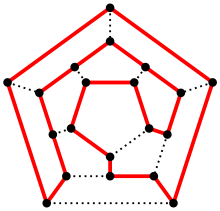
\includegraphics[width=0.25\textwidth]{tikz/hamilt.png}
  \caption{一個 Hamiltonian cycle}
\end{figure}


\subsection{匹配問題}
一個圖的匹配是一個邊集 $E'$,滿足 $E' \subseteq E$ 且每個在圖上的點至多只跟
$E'$ 裡面的一條邊相鄰。一個最大匹配就是 $\abs{E'}$ 最大的一個匹配。

\begin{figure}[H]
  \centering
  \begin{tikzpicture}[x=1.3cm,y=-1.3cm]
  \foreach \x/\y/\lab in {
    0/0/1,
    0.8/-1.3/2,
    1.2/-0.3/3,
    1.2/0.9/4,
    2.5/-0.5/5,
    2.7/0.8/6,
    -0.4/-0.9/7%
  } {
    \node[vertex, inner sep=0pt, minimum size=.7cm] (\lab) at (\x, \y) {};
  }
  \begin{scope}[every edge/.append style={pos=.5}]
    \foreach \u/\v in {
      1/2,
      1/3,
      1/4,
      2/3,
      2/5,
      3/4,
      3/5,
      3/6,
      4/5,
      5/6,
      7/1,
      7/2%
    }{
      \draw[draw,thick] (\u) edge (\v);
    }
  \end{scope}

  \begin{scope}[every edge/.append style={line width=1mm}]
    \foreach \u/\v in {
      2/3,
      4/5,
      7/1%
    }{
      \draw[draw,thick] (\u) edge (\v);
    }
  \end{scope}

\end{tikzpicture}

  \caption{一個匹配的例子}
\end{figure}

\subsubsection{二分圖上的匹配問題}
二分圖上的最大匹配可以直接轉成最大流問題求解
\footnote{可以參考「最大流」那一章}。我們這邊用另一種看法來看。
首先我們定義何謂交錯路徑。
\begin{theorem}[定義]
  一個{\bf 交錯路徑}是一個路徑 $P = (x_1, y_1, x_2, y_2, \dots, x_n, y_n)$,滿足
  \begin{itemize}
    \item 路徑上的每一條邊都在原圖的邊上。
    \item $x_1, y_n$ 都還沒有被匹配。
    \item $(y_k, x_{k+1})$ 都是已經在匹配中的邊。
    \item $(x_k, y_{k})$ 都是還沒有在匹配中的邊。
  \end{itemize}
  找到一條交錯路徑後,把 $(y_k, x_{k+1})$ 共 $n-1$ 個從匹配中移除,
  並把 $(x_k, y_k)$ 加進匹配中,就是一個大小多 $1$ 的新匹配。
\end{theorem}

\begin{figure}[H]
  \centering
  \begin{tikzpicture}[x=1.1cm,y=-1.1cm]
  \foreach \x/\y/\name/\lab in {
    0/0/$v_1$/v1,
    1/0/$v_2$/v2,
    2/0/$v_3$/v3,
    3/0/$v_4$/v4,
    0/2/$u_1$/u1,
    1/2/$u_2$/u2,
    2/2/$u_3$/u3,
    3/2/$u_4$/u4%
  } {
    \node[vertex] (\lab) at (\x, \y) {\name};
  }
  \begin{scope}[every edge/.append style={pos=.5},
    bold/.append style={line width=1mm}]
    \foreach \u/\v/\style in {
      v1/u1/{},
      v1/u2/{bold},
      v2/u2/{},
      v3/u1/{bold},
      v3/u2/{},
      v3/u3/{},
      v4/u3/{},
      v4/u4/{bold}%
    }{
      \draw[draw,thick] (\u) edge[apply style/.expand once=\style] (\v);
    }
  \end{scope}
\end{tikzpicture}
\hspace*{1cm}
\begin{tikzpicture}[x=1.6cm,y=-1.2cm]
  \foreach \x/\y/\name/\lab in {
    0/0/$v_2$/1,
    1/0/$u_2$/2,
    2/0/$v_1$/3,
    3/0/$u_1$/4,
    4/0/$v_3$/5,
    5/0/$u_3$/6%
  } {
    \node[vertex] (\lab) at (\x, \y) {\name};
  }
  \begin{scope}[every edge/.append style={pos=.5},
    bold/.append style={line width=1mm}]
    \foreach \u/\v/\style in {
      1/2/{},
      2/3/{bold},
      3/4/{},
      4/5/{bold},
      5/6/{}%
    }{
      \draw[draw,thick] (\u) edge[apply style/.expand once=\style] (\v);
    }
  \end{scope}
\end{tikzpicture}

\end{figure}

可以證明一個匹配是最大匹配的條件就是圖上已經不存在交錯路徑,因此我們可以
不斷的建一棵{\bf 交錯樹},找交錯路徑增加匹配大小,
直到不存在交錯路徑為止。詳細的證明和方法用
flow 的角度來看非常清楚,我們就不再細講。

\subsubsection{一般圖上的匹配問題}
和二分圖相似,不斷的找交錯路徑擴充。不過不同的是二分圖的交錯路徑 \\
$P = (x_1, y_1, x_2, y_2, \dots, x_n, y_n)$ 剛好有 
$x_i \in X, y_i \in Y$,其中 $X, Y$ 是二分圖的一個二分子集(也就是
$X, Y$ 各自裡面都沒有邊)。一般圖就沒有這種好事了,會造成交錯樹沒有那麼
好建,會有{\bf 花(Blossom)}的存在。

這時候就要修改演算法成{\bf 縮花演算法(Blossom Algorithm)},不過縮花演算法
蠻難寫的,最好是準備一份放在 Codebook 
\footnote{或許有人不知道,ACM-ICPC 比賽每個隊伍都可以帶約 25 頁單面的 code。}
裡。

當點數如果不大,可以直接用 $\ord{2^V V^2}$ 狀態壓縮 DP 來解。

\subsubsection{帶權匹配問題}
有時候邊上會有權重,你要找一組邊權總合最大的匹配。

在二分圖可以直接轉成 Cost-flow 來做,也有從 Dual problem 下手的演算法如
Hungarian algorithm 。

在一般圖上也有多項式時間的演算法,不過出名的難寫。有一種奇妙的假解是
基於以下觀察
\begin{theorem}[定義]
  一個最大帶權匹配中的負環定義為一個交錯環\\
  $P = (x_1, y_1, x_2, y_2, \dots, x_n, y_n, x_1)$,滿足
  \begin{itemize}
    \item $(y_k, x_{k+1}) \; \forall k$ 和 $(y_n, x_1)$ 都是已經在匹配中的邊,
      把這些邊的權重和叫作 $C_1$。
    \item $(x_k, y_{k})$ 都是還沒有在匹配中的邊,
      把這些邊的權重和叫作 $C_2$。
    \item $C_2 > C_1$
  \end{itemize}
  找到一個負環後,把上面 $n$ 個已匹配邊從匹配中移除,
  其它 $n$ 個加到匹配裡,那新的匹配的權重和更大。
\end{theorem}
發揮創意不斷的找負環直到沒有,就是一個最大帶權匹配了。

\SampleProblem{中國郵差問題}{
  給你一個圖,邊上有權重代表路徑長,你要找一個路徑,
  經過所有的邊至少一次(可以重複走),最後回到出發點,問最短的路徑長。
}
這個有點像歐拉迴路,可是每個邊可以重複經過。想法是想辦法把圖上的奇點都「補」成
偶點。如果補兩個奇點 $(u, v)$,那這兩個點的度數都加 $1$ 變成偶點,
而當然是補一條 $u \leadsto v$ 的最短路徑最賺。因此其實我們就是要把所有奇點
兩兩配對,$(u, v)$ 配對的花費就是他們之間的最短路。 

總結以上,要做的事情就是把所有奇點對 $(u, v)$ 的最短路徑求出,建成一個完全圖,
然後做最小帶權匹配,可以把邊權取負號,就變成最大帶權匹配。

\subsubsection{一些相關的問題}
我們這邊列了一些相關的問題。
\begin{description}[leftmargin=*]
  \item[最大獨立點集] 一個最大的點集 $V'$ 使得裡面的點都不相鄰。其大小記做 $I(G)$。
  \item[最大匹配數] 前面定義過了。其大小記做 $M(G)$。
  \item[最小點覆蓋] 最小的一個點集,使得所有的邊都至少與點集裡的
    一個點相鄰。\\其大小記做 $C_v(G)$。
  \item[最小邊覆蓋] 最小的一個邊集,使得所有的點都至少與邊集裡的
    一個邊相鄰。\\其大小記做 $C_e(G)$。
\end{description}

\begin{figure}[H]
  \centering
  \begin{subfigure}[b]{0.32\textwidth}
\begin{tikzpicture}[x=1.3cm,y=-1.3cm]
  \foreach \x/\y/\lab/\fl in {
    0/0/1/0,
    0.8/-1.3/2/0,
    1.2/-0.3/3/0,
    1.2/0.9/4/70,
    2.5/-0.5/5/0,
    2.7/0.8/6/70,
    -0.4/-0.9/7/70%
  } {
    \node[vertex, inner sep=0pt, fill=black!\fl, minimum size=.7cm] (\lab) at (\x, \y) {};
  }
  \begin{scope}[every edge/.append style={pos=.5}]
    \foreach \u/\v in {
      1/2,
      1/3,
      1/4,
      2/3,
      2/5,
      3/4,
      3/5,
      3/6,
      4/5,
      5/6,
      7/1,
      7/2%
    }{
      \draw[draw,thick] (\u) edge (\v);
    }
  \end{scope}
\end{tikzpicture}
\caption{獨立點集}
\end{subfigure}
%
\begin{subfigure}[b]{0.32\textwidth}
\begin{tikzpicture}[x=1.3cm,y=-1.3cm]
  \foreach \x/\y/\lab/\fl in {
    0/0/1/70,
    0.8/-1.3/2/70,
    1.2/-0.3/3/70,
    1.2/0.9/4/0,
    2.5/-0.5/5/70,
    2.7/0.8/6/0,
    -0.4/-0.9/7/0%
  } {
    \node[vertex, inner sep=0pt, fill=black!\fl, minimum size=.7cm] (\lab) at (\x, \y) {};
  }
  \begin{scope}[every edge/.append style={pos=.5}]
    \foreach \u/\v in {
      1/2,
      1/3,
      1/4,
      2/3,
      2/5,
      3/4,
      3/5,
      3/6,
      4/5,
      5/6,
      7/1,
      7/2%
    }{
      \draw[draw,thick] (\u) edge (\v);
    }
  \end{scope}
\end{tikzpicture}
\caption{點覆蓋}
\end{subfigure}
%
\begin{subfigure}[b]{0.32\textwidth}
\begin{tikzpicture}[x=1.3cm,y=-1.3cm]
  \foreach \x/\y/\lab in {
    0/0/1,
    0.8/-1.3/2,
    1.2/-0.3/3,
    1.2/0.9/4,
    2.5/-0.5/5,
    2.7/0.8/6,
    -0.4/-0.9/7%
  } {
    \node[vertex, inner sep=0pt, minimum size=.7cm] (\lab) at (\x, \y) {};
  }
  \begin{scope}[every edge/.append style={pos=.5}]
    \foreach \u/\v in {
      1/2,
      1/3,
      1/4,
      2/3,
      2/5,
      3/4,
      3/5,
      3/6,
      4/5,
      5/6,
      7/1,
      7/2%
    }{
      \draw[draw,thick] (\u) edge (\v);
    }
  \end{scope}

  \begin{scope}[every edge/.append style={line width=1mm}]
    \foreach \u/\v in {
      2/3,
      4/3,
      5/6,
      1/7%
    }{
      \draw[draw,thick] (\u) edge (\v);
    }
  \end{scope}
\end{tikzpicture}
\caption{邊覆蓋}
\end{subfigure}

\end{figure}
這些問題是很有相關性的,有以下定理:
\begin{theorem}
  對於連通圖,有
  \begin{itemize}
      \item $I(G) + C_v(G) = \abs{V}$. 
        \listeqn \label{eq:m1}
      \item $M(G) + C_e(G) = \abs{V}$.
        \listeqn \label{eq:m2}
      \item 對連通二分圖,有 $M(G) = C_v(G), I(G) = C_e(G)$.
        \listeqn \label{eq:m3}
  \end{itemize}
\end{theorem}

\begin{proof}
  對 \eqref{eq:m1} 我們證明一個獨立點集 $U$ 的補集 $U^c$ 一定是一個點覆蓋。對於所有邊 $(u, v)$,
  可知 $u, v$ 至少有一個不在 $U$,也就是在 $U^c$,因此 $U^c$ 覆蓋所有邊。
  這也同時證明了一個點覆蓋 $U$ 的補集 $U^c$ 一定是一個獨立點集。因此 $I(G) + C_v(G) = \abs{V}$。

  對 \eqref{eq:m2} ,我們先證明 $C_e(G) \leq \abs{V} - M(G)$。先找一個最大匹配 $M$,
  注意到 $M$ 恰好蓋住了 $2\abs{M} = 2 M(G)$ 個點,又因圖連通,可再找 $\abs{V} - 2 M(G)$
  個邊就把所有點都蓋住了,因此 $C_e(G) \leq \abs{V} - 2 M(G) + M(G) = \abs{V} - M(G)$。

  我們再證明 $C_e(G) \geq \abs{V} - M(G)$,也就是 $M(G) \geq \abs{V} - C_e(G)$。
  先找一個最小邊覆蓋。這些邊(加上端點)會形成許多連通塊,而對於任一個連通塊,不會有環
  ,否則隨便拔掉一條環上的邊仍可覆蓋所有點,也就是每個連通塊都是一棵樹。而每一個連
  通塊任選一條邊,這些選出來的邊都不相鄰,所以是一個匹配。假設連通塊分別為
  $S_1, S_2, \dots, S_n$,有 $V(S_1) = E(S_1) + 1$。因此
  \[ M(G) \geq n = \sum V(S_i) - E(S_i) = \sum V(S_i) - \sum E(S_i) = \abs{V} - C_e(G) \]
  
  最後證 \eqref{eq:m3}。首先對於一個匹配 $M$ 中的任一個邊,點覆蓋一定要蓋住其中一點,
  因此 $C_v(G) \geq M(G)$。 現在如果有一個圖 $G$ 滿足 $C_v(G) > M(G)$,找 $\abs{V}, \abs{E}$
  最小的一個反例。容易證明 $G$ 不是一條路徑或是一個環,因此有一個點 $u$ 的度數至少是 $3$。
  假設 $u$ 和 $v_1, v_2, v_3$ 相鄰,如果 $G_1 = G \setminus v_1$ 的最大匹配數 $M(G_1) < M(G)$,
  則因 $C_v(G_1)$ 至少是 $C_v(G) - 1$,有 $M(G_1) \leq M(G) - 1 < C_v(G_1)$,與反例的最小性
  矛盾。因此存在一個最大匹配 $M$ 使得 $v_1 \notin M$。而 $(u, v_2), (u, v_3)$ 至少有一個
  不在 $M$ 中,假設是 $e = (u, v_2)$,那考慮 $G_2 = G \setminus e$ 的最小覆蓋 $C$,由反例的最小
  性有 $M(G) = M(G_2) = C_v(G_2)$,且因為對於一個匹配 $M$ 中的任一個邊,點覆蓋一定要蓋住其中一點,
  $v_2 \notin C$,從而 $u \in C$ 所以 $C$ 也是 $G$ 的覆蓋,$M(G) = C_v(G)$,矛盾。因此
  \eqref{eq:m3} 成立。
\end{proof}

\eqref{eq:m3} 的證明其實沒有給出一個構造點覆蓋的方法,實際的構造方法有些複雜,可以
參考 Wiki。

\subsection{圖的計數問題}
有時候也有一些圖的計數問題出現,比如說

\SampleProblem{二元樹的數量}{
  求 $n$ 個點可以形成多少種不同的有根二元樹。
}
不少計數問題可以用遞迴的方式想,比如這題,不妨先想想何謂一個二元樹?
其實就是「根節點有兩個二元子樹的樹」。因此我們可以寫出遞迴式,令
$f(n)$ 表示 $n$ 個點的二元樹個數,有
\[ f(n) = \sum_{k = 0}^{n-1} f(n-k-1) f(k) , \quad f(0) = 1\] 

對組合熟悉的讀者應該一眼就可以看出這個就是著名的{\bf 卡特蘭數}。

以下也是一個類似的題目
\SampleProblem{樹的數量}{
  求 $n$ 個有編號的點可以形成多少種不同的樹。
}

這個是非常經典的問題,答案是 $n^{n-2}, n = \abs{V}$,證明如下:
\begin{proof}
  我們現在對於一棵樹,都把他轉成一個序列,過程如下。

  每次找編號最大的一個樹葉(也就是 degree 是 $1$ 的點) $u$,假設他連出去的邊是 $(u, v)$
  ,就記下 $v$ 的編號。重複 $\abs{V}-1$ 次後就只剩一個點了。

  假設得出的序列是 $(a_1, a_2, \cdots, a_{n-1}), n = \abs{V}$,注意到 $a_{n-1}$ 必定是 $1$,
  所以我們不妨只看 $(a_1, a_2, \cdots, a_{n-2})$,其中 $a_i$ 可以是 $1$ 到 $n$ 的任何數字。
  我們只要能證明一個樹可以一對一到一個這樣的序列,一個這樣的序列也一定可以還原成一棵樹即可。

  注意到如果 $\deg(v) = k$,那 $v$ 就會在序列中出現 $k-1$ 次。當兩個樹 $T_1, T_2$ 對
  應到的序列 $A_1, A_2$ 相同,如果 $\abs{T_1} = 2$,那這兩個樹肯定相同。 接下來我們用數學歸納法,
  假設這兩個樹的大小為 $k$,現在考慮他們編號最小的葉子 $u_1, u_2$,一定有 $u_1 = u_2$,
  否則假設 $u_1 < u_2$ ,那 $u_1$ 不會出現在 $a_1$ 裡但不會出現在 $a_2$ 理。
  接著因為序列的第一項相同,$u_1, u_2$ 也要接到相同的點,拔掉這個點後由歸納假設,兩棵樹仍相同,
  因此 $T_1 = T_2$,也就是不同的樹會對應到不同的序列。

  還原的方法也很簡單,如果 $n = 2$ 那只有一種可能的樹,就是 $1, 2$ 接在一起。
  假設我們要還原 $n = k$,也就是序列 $A$ 長度是 $k - 2$,我們找最小的編號 $u$ 使得
  $u$ 沒有出現在 $A$ 裡,先遞迴建出 $A' = (a_2, a_3, \dots, a_n)$ 的樹,把 $u$ 接
  上 $a_1$ 即可。

  總結以上,生成樹的個數就和序列的個數一樣,容易計算這樣的序列有 $n^{n-2}$ 種!
\end{proof}

再看一個比較不一樣的題目
\SampleProblem{三角形的數量}{
  給一個圖,求有多少點對 $(v_1, v_2, v_3)$ 滿足 $(v_1, v_2), (v_2, v_3), (v_3, v_1) \in E$。
}

如果直接枚舉 $v_1, v_2, v_3$ 是個 $\ord{V^3}$ 的做法,但聰明一點的做法是
枚舉所有邊 $(v_1, v_2) \in E$,再枚舉所有點 $v_3$,是 $\ord{VE}$。

更甚著,可以發現不需要枚舉所有點 $v_3$,只要枚舉比如 $v_2$ 所有的鄰居就可以了,
我們挑 $k = \sqrt{\abs{E}}$,再枚舉三角形的時候如果 $(v_1, v_2, v_3)$ 的度數都比
$k$ 大,我們就直接用第一種方法枚舉,注意到這種點只會有 $\ord{\sqrt{E}}$ 個,所以
複雜度是 $\ord{E \sqrt{E}}$。接下來用第二種方法枚舉,對一個邊 $(v_1, v_2)$,如果
$\deg(v_1) > k, \deq(v_2) > k$ 就捨棄,如果有一個,假設是 $v_2, \deg(v_2) < k$,
我們就再枚舉 $v_2$ 的鄰居,複雜度是 $\ord{E \sqrt{E}}$。

因此三角形有一個點的度數比 $k$ 小,一定會再上面被枚舉到,全部都比 $k$ 大我們第一
種方法也枚舉到了,經過適當的排容,總複雜度是 $\ord{E \sqrt{E}}$。

去年的講義資料分治(Square root method)有更詳細的說明。

\subsection{其它的問題}
前面講了那麼多種圖論的問題,可以發現圖論問題真的是非常豐富!
在程式競賽中更可能會出現其它奇奇怪怪的問題,這時候就只能見招拆招了!
如下面這一題

\SampleProblem[ACM ICPC Taipei regional pI]{怪圖怪題}{ 
  一個 Union-Join graph 定義為
  \begin{itemize}
    \item 一個點 $v$ 是一個 Union-Join graph.
    \item 如果 $G, H$ 都是 Union-Join graph,那他們的 Union 
      \[ G \cup H = (V(G) \cup V(H), E(G) \cup E(H)), \]
      也是 Union-Join graph.
    \item 如果 $G, H$ 都是 Union-Join graph,那他們的 Join 
      \[ G \oplus H = (V(G) \cup V(H), E(G) \cup E(H) \cup E'), \]
      其中$E' = \{(u, v) : \forall u \in G, v \in H\}$
      也是 Union-Join graph.
  \end{itemize}

  現在給你一個 Union-Join graph,你要把每一個點填上一個數字 $c(v)$,使得
  如果兩個點 $u, v$ 的數字相同,那任何 $u \leadsto v$ 的路徑上,
  都要有一個點 $w$ 使得 $c(w) < c(u)$。問你至少要用幾個不同的數字。
}

乍看之下題目無比複雜,但越複雜的題目可能反而是越簡單的題目!首先觀察到這個
圖是{\bf 被遞迴}的定義出來的,因此我們不妨就猜測,假設最少需要的數字數量是
$\tau(G)$,如果 $G = G_1 \cup G_2$,那 $\tau(G) = \tau_\cup(G_1, G_2)$,
且如果 $G = G_1 \oplus G_2$,那 $\tau(G) = \tau_\oplus(G_1, G_2)$。
我們只需要求出 $\tau_\cup, \tau_\oplus$ 這兩個函數是怎麼樣的函數就可以了。

顯然 $\tau_\cup(G_1, G_2) = \max(\tau(G_1), \tau(G_2))$,因為 Union 其實就只
是把兩張圖擺在一起而已,彼此互不影響。至於 $\tau_\oplus$ 比較複雜,觀察後可以
發現
\begin{enumerate}
  \item  兩邊的點不能有相同的數字,不然 union 就把兩個相同的數字連起來了。
  \item  Union後只有一邊裡的點可以有相同的數字,另一邊內的點一定要全不相同。
          不然如果 $G_1$ 中 $u_1, u_2$ 相同, $G_2$ 中 $v_1, v_2$ 相同,
          如果 $c(u_1) < c(v_1)$,union 後會有路徑
        $u_1 \to v_1 \to u_2$ 不符合要求,反之亦然。
\end{enumerate}
因此由上面討論我們猜想 $\tau_\oplus(G_1, G_2) = \min(\tau(G_1)+\abs{V(G_2)}, 
\tau(G_2)+\abs{V(G_1)})$。
由 1. 2. 知道這是下界,而一邊的點 (假設是 $G_1$) 選 $1, 2, \cdots, \abs{V(G_1)}$,一
邊令 $c(v) = c'(v) + V(G_1)$ 其中 $c'(v)$ 是原先的答案,顯然是一組解,因此這個答案是正確的。


\section{習題}

    \ExerciseProblem[經典問題]{樹上模 $m$ 的最長路徑}{
      給一個邊有權的樹,求一個路徑使得路徑上權值和模 $m$ 下最大。 $\cons{\abs{V} \leq 10^5}$
    }

    \ExerciseProblem[IOI 2007 Day 2]{Training}{
      給你一個帶權的圖和他的一個生成樹,你要找一個權重和最小的邊集使得
      原本的圖去掉這個邊集後沒有偶環。每個點的度數至多是 $10$。
      $\cons{\abs{V} \leq 1000, \abs{E} \leq 5000}$
    }

    \ExerciseProblem[Codeforces 223E]{Planar Graph}{
      給一個連通的平面圖,每次會給你圖上的一個環 $C_i$,問你環內有幾個點。\\
      $\cons{\abs{V} \leq 10^5, \sum \abs{C_i} \leq 10^5}$
    }

    \ExerciseProblem{競賽圖}{
      對於一個競賽圖,請證明
      \begin{enumerate}
        \item 一定存在一個點 $v$,使得對於其它點 $v$,要嘛 $u \to v$ 有邊,要嘛
          存在一個點 $w$,使得 $u \to w \to v$ 可以通。
        \item 如果不存在一個點 $v$ 使得他贏過所有人,也就是不是所有 $u$, $v \to u$
          都有邊,並也不存在一個點輸給所有其它人,則存在 Hamiltonian cycle.
      \end{enumerate}
    }

    \ExerciseProblem[NTUJ 2045]{Strygwyr, the Bloodseeker}{
      給你一個競賽圖,你要找一個 Hamiltonian path,使得假設這一個 path 為\\
      $v_1, v_2, \dots, v_n, n = \abs{V}$,對於所有 $i < j$,都存在一個
      長度不超過 $2$ 的路徑 $v_i \leadsto v_j$。
      $\cons{\abs{V} \leq 10^5}$
    }


    \ExerciseProblem[TIOJ 1692]{道路巡邏問題}{
      給你一個圖,用最少的一筆劃路徑把整個圖的邊都走過。
      $\cons{\ord{V + E}}$。
    }

    \ExerciseProblem{Hamiltonian Path}{
      請證明如果圖中所有點的度數都比 $\ceil{\abs{V}/2}$ 大,則存在 Hamiltonian path.
    }

    \ExerciseProblem[NTUJ 2061]{Halin Graph}{
      一個 Halin graph 就是一個畫在平面上的樹,然後把所有葉子用順時針依序連起來,
      最後一個葉子再連到第一個葉子。 一個 $3$-regular graph 就是每個點的 degree
      都是 $3$。給你一個邊有權的 3-regular Halin Graph,求一個權值最大的 Hamiltonian
      graph $\cons{\abs{V} \leq 10^5, \abs{E} \leq 1.5 \cdot 10^5}$
    }

    \ExerciseProblem[PA 2012]{Tax}{
      給你一個圖 $G$ ,每個點上有權重 $c(v)$,你要從 $s$ 走到 $t$,每走一條邊 $(u, v)$
      你就要付 $\max(c(u), c(v))$ 元,問你最小花費。 $\cons{\abs{V} \leq 1000, \abs{E} \leq 10^5}$
    }

    \ExerciseProblem[ASC 45 pF]{Flights}{
      給你一個圖,其中 $v_1$ 與所有其它點相鄰。你要給每個邊一個 $1, 2, \dots, \abs{E}$
      的數字,滿足令 $f(v)$ 表示所有與 $v$ 相鄰的邊的權重和,你要讓所有 $f(v)$ 都不同。
      $\cons{\abs{V} \leq 10^5, \abs{E} \leq 2 \cdot 10^5}$
    }

    \ExerciseProblem[Codeforces 600F]{Edge coloring of bipartite graph}{
      給你一個二分圖,求他最小的一個邊著色。 $\cons{\abs{V} \leq 2000, \abs{E} \leq 10^5}$
    }

    \ExerciseProblem[ASC 47 pF]{Four Colors}{
      現在有一棵樹,$A, B$ 兩個人玩一個遊戲,$A$ 先開始輪流選一個還沒有塗色的點塗成 $4$ 種顏色的
      其中一種,但相鄰的兩個點不能塗同一種顏色。如果一個人不能行動遊戲就結束。
      遊戲結束時所有的點都被塗色的話 $A$ 贏,否則 $B$ 贏。問 $A$ 的必勝策略?
    }


    \ExerciseProblem{同色三色形}{
      給你一個完全圖,圖的邊不是黑色就是白色,問你有幾個同色三角形。 $\cons{\ord{\abs{V}^2}}$
    }

    \ExerciseProblem[POJ 1737]{Conntected Graph}{
      問你 $n$ 個有編號的點可以形成多少不同的連通圖。 $\cons{n \leq 50}$
    }


    \ExerciseProblem[NTUJ 2539]{Drawing Hell}{
      給你一個平面圖,兩個人玩一個遊戲,輪流連一條邊,但邊不可以和已經在圖上的
      邊相交(只能在點上)。問先手還是後手贏。
      $\cons{\abs{V} \leq 10^3}$
    }

    \ExerciseProblem[ASC 41 pB]{Bicoloring of a tree}{
      給你一棵樹,樹上有 $2n$ 個點,並且沒有一個點的度數超過 $n$。現在
      你要用 $n+1$ 個顏色塗色,使得
      \begin{itemize}
        \item 兩個相鄰的點都不同色。
        \item 一個顏色至多塗兩個點。
        \item 用 $f(v)$ 表示點 $v$ 塗的顏色,不存在兩個邊 $(u_1, v_1), (u_2, v_2)$,
          使得 $(f(u_1), f(v_1)) = (f(u_2), f(v_2))$ 或是
          $(f(u_1), f(v_1)) = (f(v_2), f(u_2))$.
      \end{itemize}
      $\cons{\abs{2n} \leq 10^5}$
    }

    \ExerciseProblem[ACM ICPC Taipei regional pE]{怪圖怪題}{
      給你一個圖,邊的距離都是 $1$,滿足所有的點雙連通元件都是完全圖。你要在裡面選
      $k$ 個點,使得這 $k$ 個點連通,並且所有點到這個點集的距離和最少。
      $\cons{\ord{kVE}}$
    }

    \ExerciseProblem[ASC 35 pF]{Graph Factorization}{
      給你一個有偶數個點的完全圖 $K_{2n}$,把他的邊分解成 $2n - 1$ 個集合,
      使得每個點在一個集合裡都只與一個邊相鄰(也就是每個集合都是一個匹配)。
      $\cons{n \leq 100}$
    }

    \ExerciseProblem[ASC 34 pI]{Tour}{
      給你一棵樹,問你要加幾條邊才會有一個 Hamiltonian Cycle。
      $\cons{\abs{V} \leq 10^5}$
    }

    \ExerciseProblem[ASC 34 pA]{Three Color}{
      給你一個二分圖 $G$,你要給每個邊一個 $0, 1, 2$ 的權值,使得令 $f(v)$ 表示一與點
      $v$ 相鄰的所有的邊的權值總合,所有 $f(v)$ 都不相同。
      $\cons{\abs{V} \leq 3000, \abs{M} \leq 10000}$
    }

    \ExerciseProblem[ASC 38 pJ]{Jackpot}{
      現在有一個圖,兩個人 $A, B$ 玩一個遊戲,輪流把圖上的一個點塗黑或白色,但
      相鄰的點不能塗同一個顏色。誰塗不了就輸了,問雙方都使用最佳策略的情況下誰贏。
      $\cons{\abs{V}, \abs{E} \leq 10^5}$
    }

    \ExerciseProblem[ASC ??]{??}{
      給你一棵樹,要加上幾條邊才可以讓整張圖雙連通?
      $\cons{\ord{V}}$
    }

  \section{Special Thanks}
  此分講義部分參考自去年及前年的講義,特別感謝以前的編輯者。
\end{document}
